%-----------------------------START OF PACKAGES-----------------------------%
\documentclass{article}

% Language setting
\usepackage[english]{babel}
\usepackage[T5]{fontenc}    
\usepackage[utf8]{inputenc} 
\usepackage{lmodern}

% Set page size and margins
\usepackage[letterpaper,top=2cm,bottom=2cm,left=3cm,right=2cm,marginparwidth=1.75cm]{geometry}

% Useful packages
\usepackage{amsmath}
\usepackage{amssymb}
\usepackage{graphicx}
\usepackage[colorlinks=true, allcolors=blue]{hyperref}
\usepackage{booktabs}
\usepackage{float}
\usepackage{placeins}
\usepackage{fix-cm}
\usepackage{tikz}  
\usepackage{array}
\usepackage{xcolor}
\usepackage{romanbar}
\usepackage{tocloft}
\usepackage{hyperref}
\usepackage{multicol}
\usepackage{makecell}
\usepackage{titlesec}
\usepackage{fix-cm}
\usepackage[backend=biber]{biblatex}
\addbibresource{bibliothaque.bib}
\usepackage{etoolbox}
%------------------------------END OF PACKAGES------------------------------%

%-----------------------------START OF SETTING------------------------------%
\DefineBibliographyStrings{english}{
  references = {REFERENCES}, % Makes the heading uppercase
}

\setcounter{secnumdepth}{4}
\setcounter{tocdepth}{4}

% Set section to uppercase Roman numerals
\renewcommand{\thesection}{\Roman{section}.}
% Subsection as Arabic
\renewcommand{\thesubsection}{\arabic{subsection}}
% Subsubsection as 1.1
\renewcommand{\thesubsubsection}{\arabic{subsection}.\arabic{subsubsection}}

% define color
\definecolor{darknavy}{RGB}{23, 54, 93}

% Define a colored rule
\definecolor{officeblue}{RGB}{79,129,189}

% Adds horizontal line after section
\titleformat{\section}
  {\color{darknavy}\normalfont\Large\bfseries}
  {\thesection}{1em}{}
  [\color{officeblue}\titlerule]  

\cftsetindents{section}{0em}{2.5em}

% Define subsubsubsection
\makeatletter
% Define subsubsubsection counter
\newcounter{subsubsubsection}[subsubsection]
\renewcommand\thesubsubsubsection{\thesubsubsection.\arabic{subsubsubsection}}

% Define the subsubsubsection command
\renewcommand\thesubsubsubsection{\thesubsubsection.\arabic{subsubsubsection}}

\newcommand\subsubsubsection[1]{%
  \refstepcounter{subsubsubsection}%
  \vspace{1.5ex plus 0.5ex}%
  {\par\noindent\normalfont\normalsize\bfseries
   \thesubsubsubsection\hspace{1em}#1\par}%
  \addcontentsline{toc}{subsubsubsection}{\thesubsubsubsection\quad #1}%
  \vspace{0.8ex plus 0.2ex}%
  \noindent\ignorespaces 
}

% Add subsubsubsection to Table of Contents
\newcommand{\l@subsubsubsection}{\@dottedtocline{4}{7em}{4em}}

% Adjust TOC depth to show subsubsubsections
\setcounter{tocdepth}{4}
\makeatother

%------------------------------END OF SETTING-------------------------------%

%----------------------------START OF TITLEPAGE-----------------------------%
\begin{document}
% Title pages
\begin{titlepage}
    % Margin
    \begin{tikzpicture}[remember picture, overlay]
        \draw[line width=4.5pt]
        ([xshift=2cm, yshift=-1.75cm]current page.north west) rectangle 
        ([xshift=-1cm, yshift=1.75cm]current page.south east);
    \end{tikzpicture}
    
    \centering
    \vspace*{1cm}

    % logo
    {\Large \bfseries UNIVERSITY OF SCIENCE AND TECHNOLOGY OF HA NOI \par}
    {\LARGE \bfseries UNDERGRADUATE SCHOOL \par}

    \begin{figure}[H]
        \centering
        
\includegraphics[width=0.50\linewidth]{logo.png}
        \label{fig:logo}
    \end{figure}

    % Title and name
    \vspace{0.75cm}
    {\LARGE \bfseries BACHELOR THESIS \par}
    \vspace{1cm}
    {\huge \bfseries TRANSFER LEARNING FOR WORD-LEVEL SIGN LANGUAGE CLASSIFICATION\par}
    \vspace{0.25cm}
    {\Large \bfseries by \par}
    \vspace{0.25cm}
    {\LARGE \bfseries LE DUC DUNG \par}
    {\LARGE \bfseries 22BI13103 - DATA SCIENCE \par}
    {\Large Academic year: 2021-2025 \par}
    \vspace{1.5cm}

    % Supervisors
    {\Large External Supervisor: \par}
    \vspace{0.15cm}
    {\LARGE \bfseries Assoc. Prof. NGUYEN DUC DUNG \par}
    {\Large Internal Supervisor: \par}
    \vspace{0.15cm}
    {\LARGE \bfseries Dr. NGHIEM THI PHUONG\par}

    % Affiliation
    \vspace{0.5cm}
    {\LARGE \bfseries Institute of Information Technology \par}

    % Date
    \vspace{1.5cm}
    {\Large \bfseries Hanoi, July 2025 \par}
\end{titlepage}
%------------------------------END OF TITLEPAGE-----------------------------%

%-----------------------------START OF DOCUMENTS----------------------------%
% Table of Contents
\tableofcontents
\newpage

% Declaration
\section*{DECLARATION}
\phantomsection
\addcontentsline{toc}{section}{DECLARATION}
\vspace{0.25cm}

I hereby certify that the thesis is my original work prepared and completed under the supervision of my supervisor Assoc. Prof. NGUYEN Duc Dung.

\vspace{0.5cm}
\noindent I certify that the work for which the results of this project have not been presented or submitted anywhere else. No part of the content of this thesis has ever been published in any form before. In addition, all consults, comments, and statistics from other authors and organizations have been cited accordingly. I shall be solely responsible if any fraud is found against my declaration.

\vspace{3cm}
\section*{LỜI CAM ĐOAN}
\vspace{0.25cm}

Tôi xin cam đoan rằng luận án này hoàn toàn là công sức của tôi được chuẩn bị và hoàn thiện dưới sự giúp đỡ và hướng dẫn của Phó Giáo sư Nguyễn Đức Dũng.

\vspace{0.5cm}
\noindent Tôi xin xác nhận rằng mọi công việc và kết quả của dự án này chưa được trình bày hoặc xuất bản ở bất kì nơi nào khác. Không một phần nội dung nào của luận án này từng được công bố dưới mọi hình thức nào trước đây. Ngoài ra, mọi sự tham khảo, nhận xét, thống kê từ các tác giả và tổ chức khác đều đã được tôi trích dẫn tương ứng. Tôi sẽ hoàn toàn chịu trách nhiệm nếu có bất kỳ gian lận nào được phát hiện.

\vspace{8cm} 
\noindent LE Duc Dung \\
\noindent University of Science and Technology of Hanoi \\
\noindent Hanoi, July 2025
\newpage

% Acknowledgment
\section*{ACKNOWLEDGMENT}
\phantomsection
\addcontentsline{toc}{section}{ACKNOWLEDGMENT}
\vspace{0.25cm}

My thesis would not be completed without the help of many people to whom I wish to express my gratitude.

\vspace{0.5cm}
\noindent I would like to express my sincere thanks to my project guide at IOIT, Assoc. Prof. NGUYEN Duc Dung for offering me a place to do an internship, and for his enthusiastic guidance, precious feedback, and constructive instruction throughout the project. He was also the person who gave me the idea for my project. In addition, I would like to
thank all my friends at USTH, Trinh Van Quyet, Nguyen Tien Cong, and Do Duy Toan for supporting me greatly with the solution during the time I was doing this project.

\vspace{0.5cm}
\noindent Finally, to my family, my friends and all the people at USTH, I really want to express my deepest gratitude for your help during my time at university. I have learned a lot and matured a lot since the first day I came here. 

\vspace{3cm}
\section*{LỜI CẢM ƠN}
\vspace{0.25cm}

Luận án của tôi sẽ không được hoàn thành nếu không có sự giúp đỡ của rất nhiều người mà tôi muốn bày tỏ lời cảm ơn chân thành nhất.

\vspace{0.5cm}
\noindent Tôi muốn gửi lời cảm ơn chân thành nhất đến người hướng dẫn của tôi ở Viện Công Nghệ Thông Tin, Phó Giáo sư Nguyễn Đức Dũng đã cho tôi vị trí thực tập, và sự hướng dẫn tận tình, những ý kiến đóng góp
quý báu và những chỉ dẫn mang tính xây dựng của thầy trong suốt thời gian thực hiện đồ án. Thầy cũng là người lên ý tưởng cho tôi cho dự án của mình. Ngoài ra, tôi muốn gửi lời cảm ơn đến tất cả bạn bè của tôi ở USTH, Trịnh Văn Quyết, Nguyễn Tiến Công, và Đỗ Duy Toàn đã hỗ trợ tôi rất nhiều về những hướng giải quyết trong suốt thời gian tôi thực hiện dự án.

\vspace{0.5cm}
\noindent Cuối cùng, gửi đến gia đình, bạn bè và tất cả tất cả con người tại USTH, tôi thực sự muốn gửi lời cảm ơn sâu sắc nhất đến sự giúp đỡ của mọi người trong suốt thời gian tôi học tại trường đại học. Tôi đã học hỏi và trưởng thành rất nhiều kể từ ngày đầu tiên đến đây

\vspace{5cm} 
\noindent LE Duc Dung \\
\noindent University of Science and Technology of Hanoi \\
\noindent Hanoi, July 2025
\newpage

% Abbreviations
\section*{LIST OF ABBREVIATIONS}
\phantomsection
\addcontentsline{toc}{section}{LIST OF ABBREVIATIONS}

\renewcommand{\arraystretch}{1.4} % vertical spacing
\vspace{1em}
\hspace*{1.55cm}
\begin{tabular}{@{}>{\bfseries}l@{\hspace{1cm}}p{15cm}}
\textbf{USTH}   & University of Science and Technology of Ha Noi \\
\textbf{WLASL}  & Word-Level American Sign Language \\
\textbf{S3D}    & Seperable 3D Convolutional Neurel Network \\
\textbf{RNNs}   & Recurrent Neural Networks \\
\textbf{CNNs}   & Convolutional Neural Networks \\
\textbf{MLP}    & Multilayer Perceptron \\
\textbf{BiGRU}  & Bidirectional Gated Recurrent Unit. \\
\textbf{STEPNET}& Spatial-temporal Part-aware Network \\
\textbf{LLMs}   & Large Language Models \\
\textbf{SLR}    & Sign Language Recognition \\
\textbf{SLN}    & S3D-LandmarkNet   \\
\textbf{SOTA}   & State Of The Art \\
\end{tabular}

\vspace{2cm}

\section*{GLOSSARY OF TERMS}
\phantomsection
\addcontentsline{toc}{section}{GLOSSARY OF TERMS}

\renewcommand{\arraystretch}{1.4} 
\vspace{1em}
\begin{tabular}{@{}>{\bfseries}l@{\hspace{0.8cm}}l@{\hspace{0.8cm}}p{10cm}@{}}
\textbf{Term}        & \textbf{Alias}      & \textbf{Definition} \\
\textbf{Landmark}    & Keypoints, Joints   & A coordinate representing a joint or feature on the human body. \\
\textbf{NSLT100}     & WLASL100            & A 100-class subset of the WLASL dataset used in experiments. \\
\end{tabular}

\newpage

\renewcommand{\listtablename}{LIST OF TABLES}
\titleformat{\listtablename}
  {\color{darknavy}\normalfont\Large\bfseries}
  {\thesection}{1em}{}
  [\color{officeblue}\titlerule] 
\addcontentsline{toc}{section}{LIST OF TABLES}
\listoftables

\vspace{2cm}

\renewcommand{\listfigurename}{LIST OF FIGURES}
\titleformat{\listfigurename}
  {\color{darknavy}\normalfont\Large\bfseries}
  {\thesection}{1em}{}
  [\color{officeblue}\titlerule]
\addcontentsline{toc}{section}{LIST OF FIGURES}
\listoffigures

\newpage

\section*{ABSTRACT}
\phantomsection
\addcontentsline{toc}{section}{ABSTRACT}
\vspace{0.25cm}

Sign Language Recognition (SLR) is a challenging topic in Computer Vision due to the complex combination of hand gestures, facial expressions, body movements, and video pre-processing techniques. This thesis proposes a fusion model that uses both video data and extracted human body landmarks (keypoints) to improve recognition performance. I introduce the S3D-LandmarkNet (SLN) Model which integrates an S3D backbone \cite{xie2017rethinking} without classification layer to extract essential spatial-temporal features from resized RGB video frames and Landmark Transformer, reconstructed based a custom-design STEPNET \cite{pan2022stepnet} architecture to process spatial-temporal features of extracted landmarks. The Landmark Transformer applies 4 components named Spatial Partition, Spatial Attention, Temporal Partition, and Temporal Attention with bidirectional GRU to process full-body landmarks (body, face and 2 hands) as well as extract motion-aware features. The video features and landmark features are fused at the end and passed through a classification layer to yield prediction for the label of sign language. My model training, validation and evaluation phases are conducted on the NSLT100 official train, validation, and test sets, also known as WLASL100 \cite{paperswithcode_wlasl100} - a subset of WLASL2000 \cite{li2020wlasl} \cite{paperswithcode_wlasl2000} with 100 classes (hearing, thank, ...) which includes a wide range of America Sign Language signs with high inter-class similarity, signer and source diversity. Experimental results show that my model achieves Top-1 accuracy of 92.47\% and Top-5 accuracy of 94.92\% (Per-instance). These results illustrate the effectiveness of combining video features and human landmark features through a temporal processing layer and attention-guided modeling. The proposed model demonstrates a robust and generalizable sign language recognition model and proves the effectiveness of the transfer learning model techniques.

\vspace{1cm}
\textbf{Keyword:} Sign Language Recognition (SLR), Spatio-Temporal Features, Landmark Transformer, S3D , Landmarks, Temporal Attention, Spatial Attention, Bidirectional GRU, Multimodal Fusion, NSLT100, WLASL, Transfer Learning, Computer Vision

\newpage

\section{INTRODUCTION}

This section provides the context and motivation for the research, clearly defines the problem being addressed, outlines the objectives, and summarizes the thesis structure.

\subsection{Context and Motivation}

Sign languages are rich visual languages that play a core role in the way of communication for millions of deaf and hard-of-hearing individuals worldwide. These languages communicate meaning through a sophisticated combination of hand gestures, hand movements, facial expressions, and body movements as well as spatial-temporal dynamics. With the need for implicit technology development, SLR has emerged as a crucial area in computer vision generally, and aiming to build a bridge for communication barriers between signers and non-signers particularly. Unlike spoken languages, in which people can directly receive linear information and response immediately, sign language seems to involve simultaneous and sequential visual cues that are often subtle and context-dependent (The similar sign between number '0' and character 'O', for example).

\vspace{0.5cm}

Traditional SLR models that rely solely on RGB images and RGB video data are limited by their lack of abilities to properly capture structural and motion-specific temporal features in sign language. Variability in signer appearance, gesture speed, and the resemblance in many signs increase the difficulties in SLR. Deep Learning models such as 3D CNNs may have improvements by learning spatial-temporal patterns from raw video data, but they still struggle when dealing with challenges in the generalization of temporal features. Moreover, video data alone may miss crucial structural patterns, especially in signs with minor visual distinctions.

\vspace{0.5cm}

To overcome these limitations, recent advancements explore approaches that integrate full-body landmark data with input data. This work is inspired and motivated by the hypothesis that a transfer learning S3D \cite{xie2017rethinking} model combining video-based and structure-based features can make progress for the model's ability to recognize signs more accurately and robustly. In this project, I propose a SLN model that fuses features extracted from an S3D \cite{xie2017rethinking} backbone with landmark-based representations processed by Landmark Transformer build based on STEPNET model \cite{pan2022stepnet}. This additional module contains spatial partitioning, attention-based encoding, and temporal modeling on landmarks of three parts: body, face, and hands. The transfer learning method enables the model to better capture the essential components of sign language and enhances recognition performance and access to diverse signs. This approach harnesses the knowledge in transfer learning, fine-tuning it for the specific task of SLR, and thereby accelerating development.

\subsection{Literature Review}
Nowadays, SLR has gained increasing attention in the fields of Computer Vision due to its potential to improve communication accessibility for deaf and hard-of-hearing communities. Traditional approaches to SLR were based on handcrafted features such as shape descriptors. However, these techniques lacked the ability to handle the temporal features and generalize across diverse signs.

\vspace{0.5cm}

With the significant development of deep learning, many researches and projects have adopted CNNs and RNNs to model spatial-temporal patterns in sign language video data. For example, 3D CNNs such as C3D \cite{tran2015learning}, I3D \cite{carreira2017quo} and S3D \cite{xie2017rethinking} - a Separable I3D model have made progress in capturing temporal patterns from raw video frames. NLA-SLR \cite{zuo2023natural} - a multimodal model using S3D and VKNet (built on HRNet \cite{sun2019deep}) and UniSign \cite{li2025uni-sign} with pretrained LLMs have shown an advancement in both capturing temporal motion and applying keypoints (landmarks) from video inputs. The 3D CNNs, I3D for instance, leverages inflated 2D kernels from ImageNet-pretrained networks to process video sequences, providing strong performance in gesture and action recognition tasks but these video-only models often struggle with ambiguous or similar-looking signs that differ mainly in hand configurations and hand movements or facial expressions. The existing video and landmark combination models required expensive computational cost with LLMs and heavy networks.

\vspace{0.5cm}

To address this problem, I choose to use other frameworks to extract structured motion landmarks such as Google Mediapipe \cite{mediapipe_holistic_landmarker} which enable landmark extraction, allowing me to explore skeletal representations of the hands, body and face. Several works have used RNNs and Transformers to model these landmark sequences and extract the temporal patterns for SLR. My proposed model extends this line of work by combining a strong spatial-temporal video backbone (S3D \cite{xie2017rethinking}) with a landmark encoder (Landmark Transformer) that applies spatial partitioning, attention and temporal modeling to sequence features. This fusion model aims to leverage the strengths of combination of visual and structural cues to improve recognition accuracy and generalization across signs.

\subsection{Main Question}
The core objective of this project is to investigate whether a multimodal deep learning framework that fuses spatial-temporal video features with structured landmark representations can enhance the performance of SLR systems. In particular, it explores how effectively a transfer learning approach enhances the performance of S3D \cite{xie2017rethinking} and the positive impact of combining video-based backbone with Landmark Transformer that encodes spatial and temporal pattern from full-body landmarks on training and evaluating on WLASL \cite{li2020wlasl} dataset. Given the complexity of sign language, where details in motion, hand shape, and facial expressions convey distant meanings, this research seeks to answer: Can integrating visual and structural motion cues improve recognition accuracy and generalization across diverse signs? The goal is not only to improve classification performance but also to demonstrate the benefits of modality fusion in addressing the challenges of SLR.

\subsection{Thesis Structure}
\textbf{Section I:} \textbf{INTRODUCTION}, provides the research context, motivation, and a review of existing methods, outlining the key questions addressed.

\vspace{0.25cm}

\noindent\textbf{Section II:} \textbf{OBJECTIVES}, defines the goals, focusing on creating a generalizable SLR system using transfer learning with video-based backbone S3D and integrating Landmark Transformer on sequence patterns extraction.

\vspace{0.25cm}

\noindent\textbf{Section III:} \textbf{MATERIALS AND METHODOLOGY}, details the datasets WSASL and WLASL100, pre-processing techniques, and the combined S3D model architecture with Landmark Transformer.

\vspace{0.25cm}

\noindent\textbf{Section IV:} \textbf{RESULTS AND DISCUSSIONS}, presents the experimental results, including performance metrics in both datasets, comparisons with other methods, and a critical analysis of the effectiveness and limitations of the approach.

\vspace{0.25cm}

\noindent\textbf{Section V:} \textbf{CONCLUSION}, summarizes the achievements, specifically the high accuracy on WLASL100 datasets, discusses limitations, and suggests future research directions.

\section{Objectives}
The core objective of this research is to develop a robust and well-performed SLR model that concludes both visual and structural information through a multimodal deep learning architecture. To achieve this, I propose combining a video-based spatiotemporal feature extractor with a landmark-based encoder that models body, hand, and facial movements. This fusion is designed to capture the expressive components of sign language that are often missed when relying solely on RGB video data.

\vspace{0.5cm}

One key goal is to utilize the transfer learning on the S3D \cite{xie2017rethinking} backbone as the backbone for extracting essential spatiotemporal features from raw video sequences. S3D \cite{xie2017rethinking} is chosen for its efficiency and strong performance in action recognition, which makes it well-suited for modeling the motion dynamics.

\vspace{0.5cm}

In addition, I aim to build a Landmark Transformer module that processes body, hand, and face keypoints using a series of operations: spatial partitioning, attention-based encoding, and temporal extraction. This module is designed to focus on the most informative parts of the human body during signing, helping the model to better recognize signs.

\vspace{0.5cm}

Another objective is to fuse the representations from both video-based model and structure-based (landmarks)—into a unified feature vector that supports more accurate recognition. And finally, this model is compared to SOTA - existing methods to state the conclusion.

\vspace{0.5cm}

Through these objectives, this research shows the enhancement of current SLR systems by demonstrating that multimodal fusion can provide deeper insight and stronger performance in real-world sign language recognition tasks.

\section{MATERIALS AND METHODOLOGY}
This section details the methodology employed, beginning with the datasets and pre-processing techniques used. The core model architecture integrates a S3D \cite{xie2017rethinking} backbone with a Landmark Transformer, incorporating a modified initial S3D classification head.

\subsection{Environment Settings}
For this research, to ensure the convenience and efficient experimentation, all model training and evaluation were conducted in a controlled computational environment. The implementation was carried out using \textbf{Python 3.10} with the \textbf{PyTorch 2.1} deep learning framework on Google Colab, which offers robust tools for dynamic computation graphs and GPU acceleration.

\vspace{0.5cm}

\noindent The primary development environment included the following key components:

\subsubsection*{Hardwares}
\begin{itemize}
  \item \textbf{CPU:} Intel(R) Xeon(R) CPU @ 2.20GHz
  \item \textbf{GPU:} NVIDIA A100-SXM4-40GB with CUDA support
  \item \textbf{RAM:} 89.6 GB
  \item \textbf{Storage:} Google Colab Cloud
\end{itemize}

\subsubsection*{Software \& Libraries}
\begin{itemize}
  \item Python 3.10
  \item PyTorch 2.1
  \item Torchvision 0.16+
  \item NumPy 1.25+
  \item OpenCV 4.x
  \item Matplotlib 3.x
  \item MediaPipe (for landmark extraction) 0.10.21
  \item Scikit-learn (for evaluation metrics and utilities) and more
\end{itemize}

\subsubsection*{Platform \& Tools}
\begin{itemize}
  \item \textbf{Operating System:} Linux-6.1.123+-x86\_64-with-glibc2.35
  \item Google Colab for prototyping
  \item TensorBoard for visualizing training logs and performance
  \item Git for version control
  \item Drawio for visualizing model architecture
\end{itemize}

All models were trained using NVIDIA GPUs with \textbf{CUDA 12.4} support to accelerate tensor computations. The deep learning pipelines, including video preprocessing, landmark extraction, and training loops, were optimized to make full use of hardware resources via \
\texttt{torch.cuda.amp} for mixed precision training. This environment setup ensured stable and efficient training while enabling reproducibility across different hardware platforms.

\subsection{Dataset}
\subsubsection{Overview}

Several publicly accessible sign language datasets have been collected in countries such as The United States, Germany and China. In this research, I utilized WLASL \cite{li2020wlasl}. This dataset is labeled and contains 21,095 videos and 2000 classes/words/glosses, collected on over 2700 sources and performed by over 100 signers, with duration in range of 0.6 and 8.1 seconds and fps from 12 to 60. There are multiple reasons for choosing this dataset over the others, including the effective use of transfer learning to reduce  computational resources and training time, as well as to demonstrate the robust effectiveness across diverse signs and to appear as the newest challenge on Word-Level Sign Language. This dataset approach was essential for comprehensive assessment of the model’s generalizability and robustness across different conditions and geographical contexts. Nowadays, a WLASL website \cite{paperswithcode_wlasl2000} is maintained, where results are still accepted, processed, and shown on a leaderboard. This rating aids in determining which are the SOTA approaches utilised for SLR.

\begin{figure}[H]
    \centering
    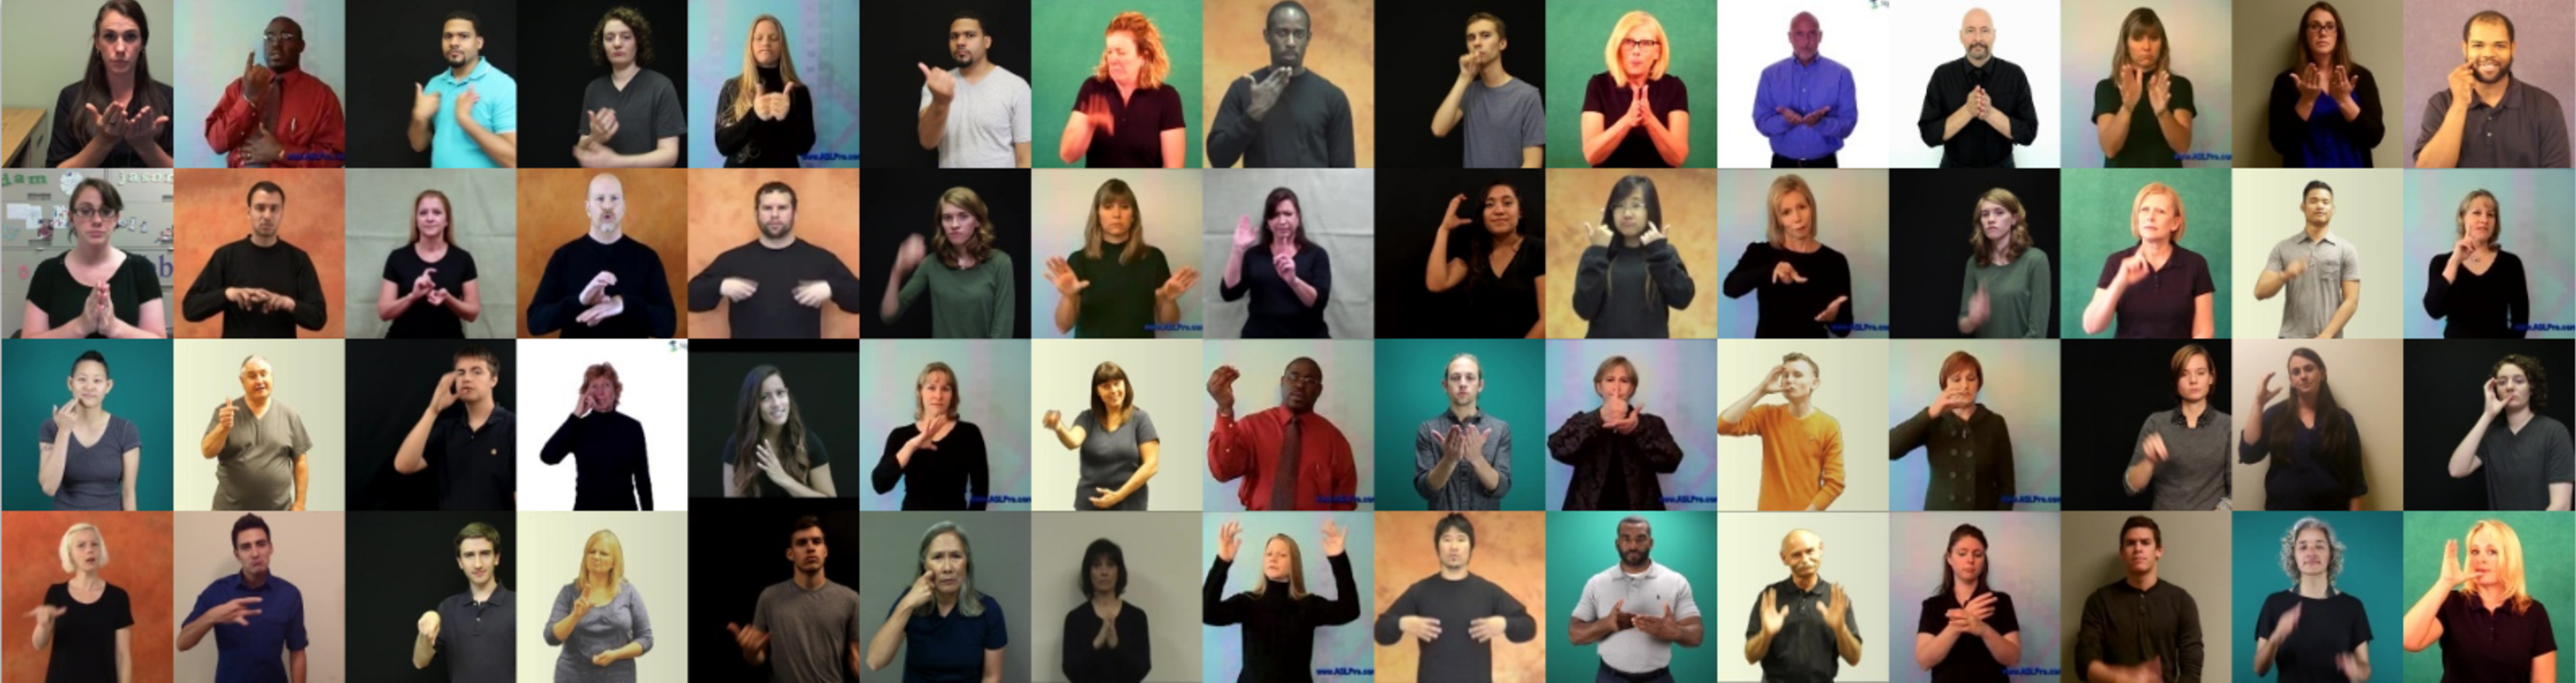
\includegraphics[width=1\linewidth]{Fig/4row.pdf}
    \caption{Samples of WLASL}
    \label{fig:wlasl}
\end{figure}

\subsubsection{NSLT100}

For this project, I selected the NSLT100 dataset, a labeled subset of the larger WLASL2000 dataset, which has 100 sign language classes and a total of 2,038 video samples. The reason for choosing this dataset is because of its smaller size, making it better for training and experimentation under shortage of my computational resources, such as those defined in my environment settings. On the contrary, WLASL2000 requires more GPU memory and training time. NSLT100 provides a balanced trade-off for my environment settings between diversity of gestures in NSLT100 and computational efficiency. This dataset also is splitted into 3 subsets: train set with 1442 samples, validation set with 338 samples and test set with 258 samples.

\begin{figure}[H]
    \centering
    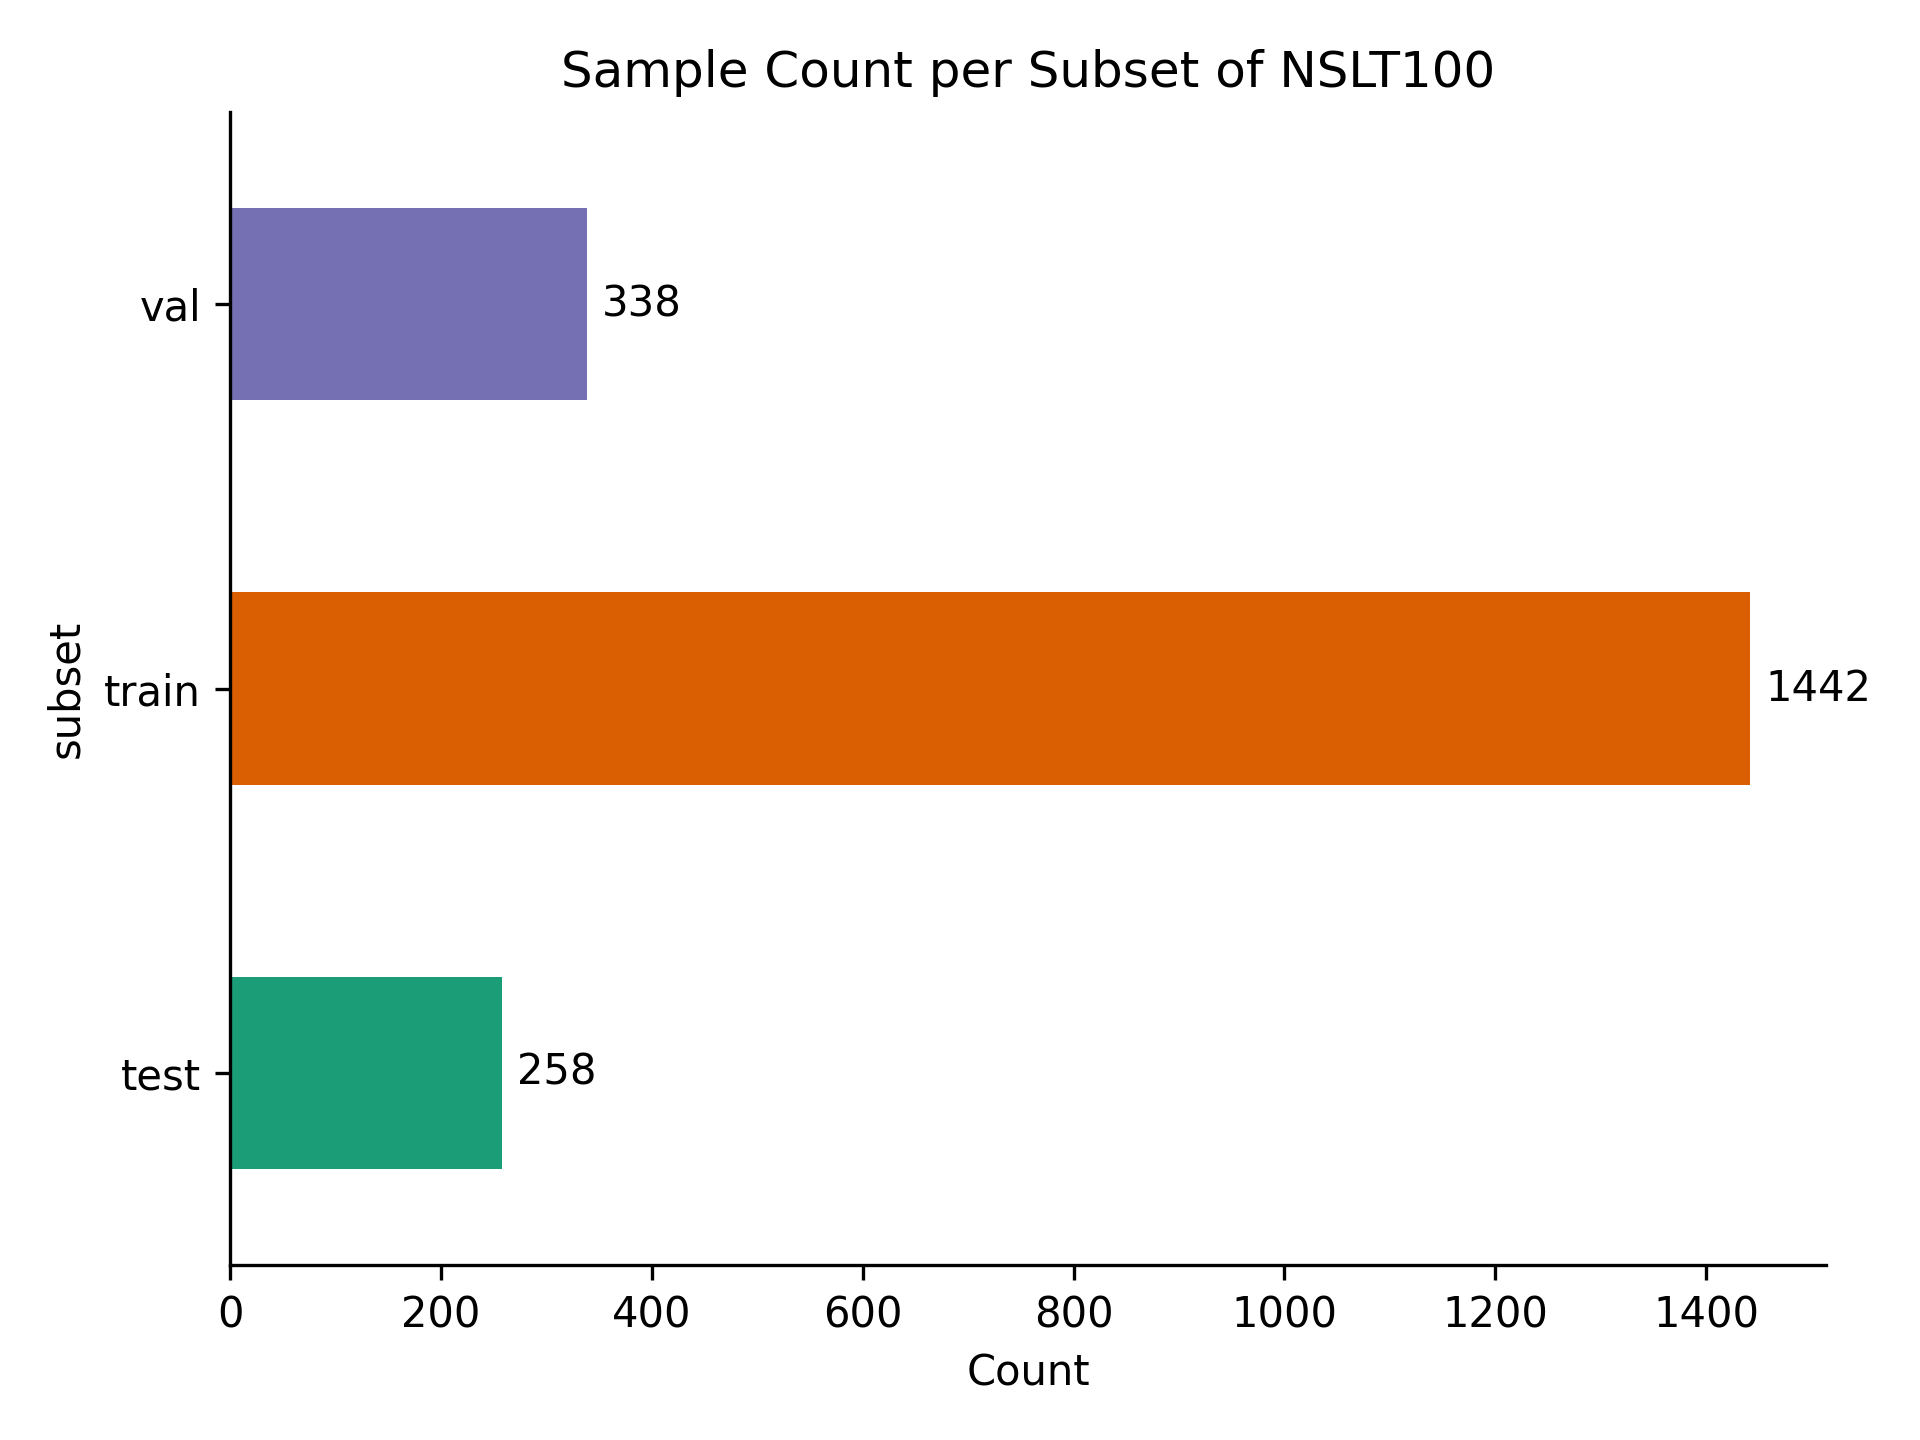
\includegraphics[width=0.65\linewidth]{Fig/split.png}
    \caption{Sample Count per Subset of NSLT100}
    \label{fig:split}
\end{figure}

\begin{figure}[H]
    \centering
    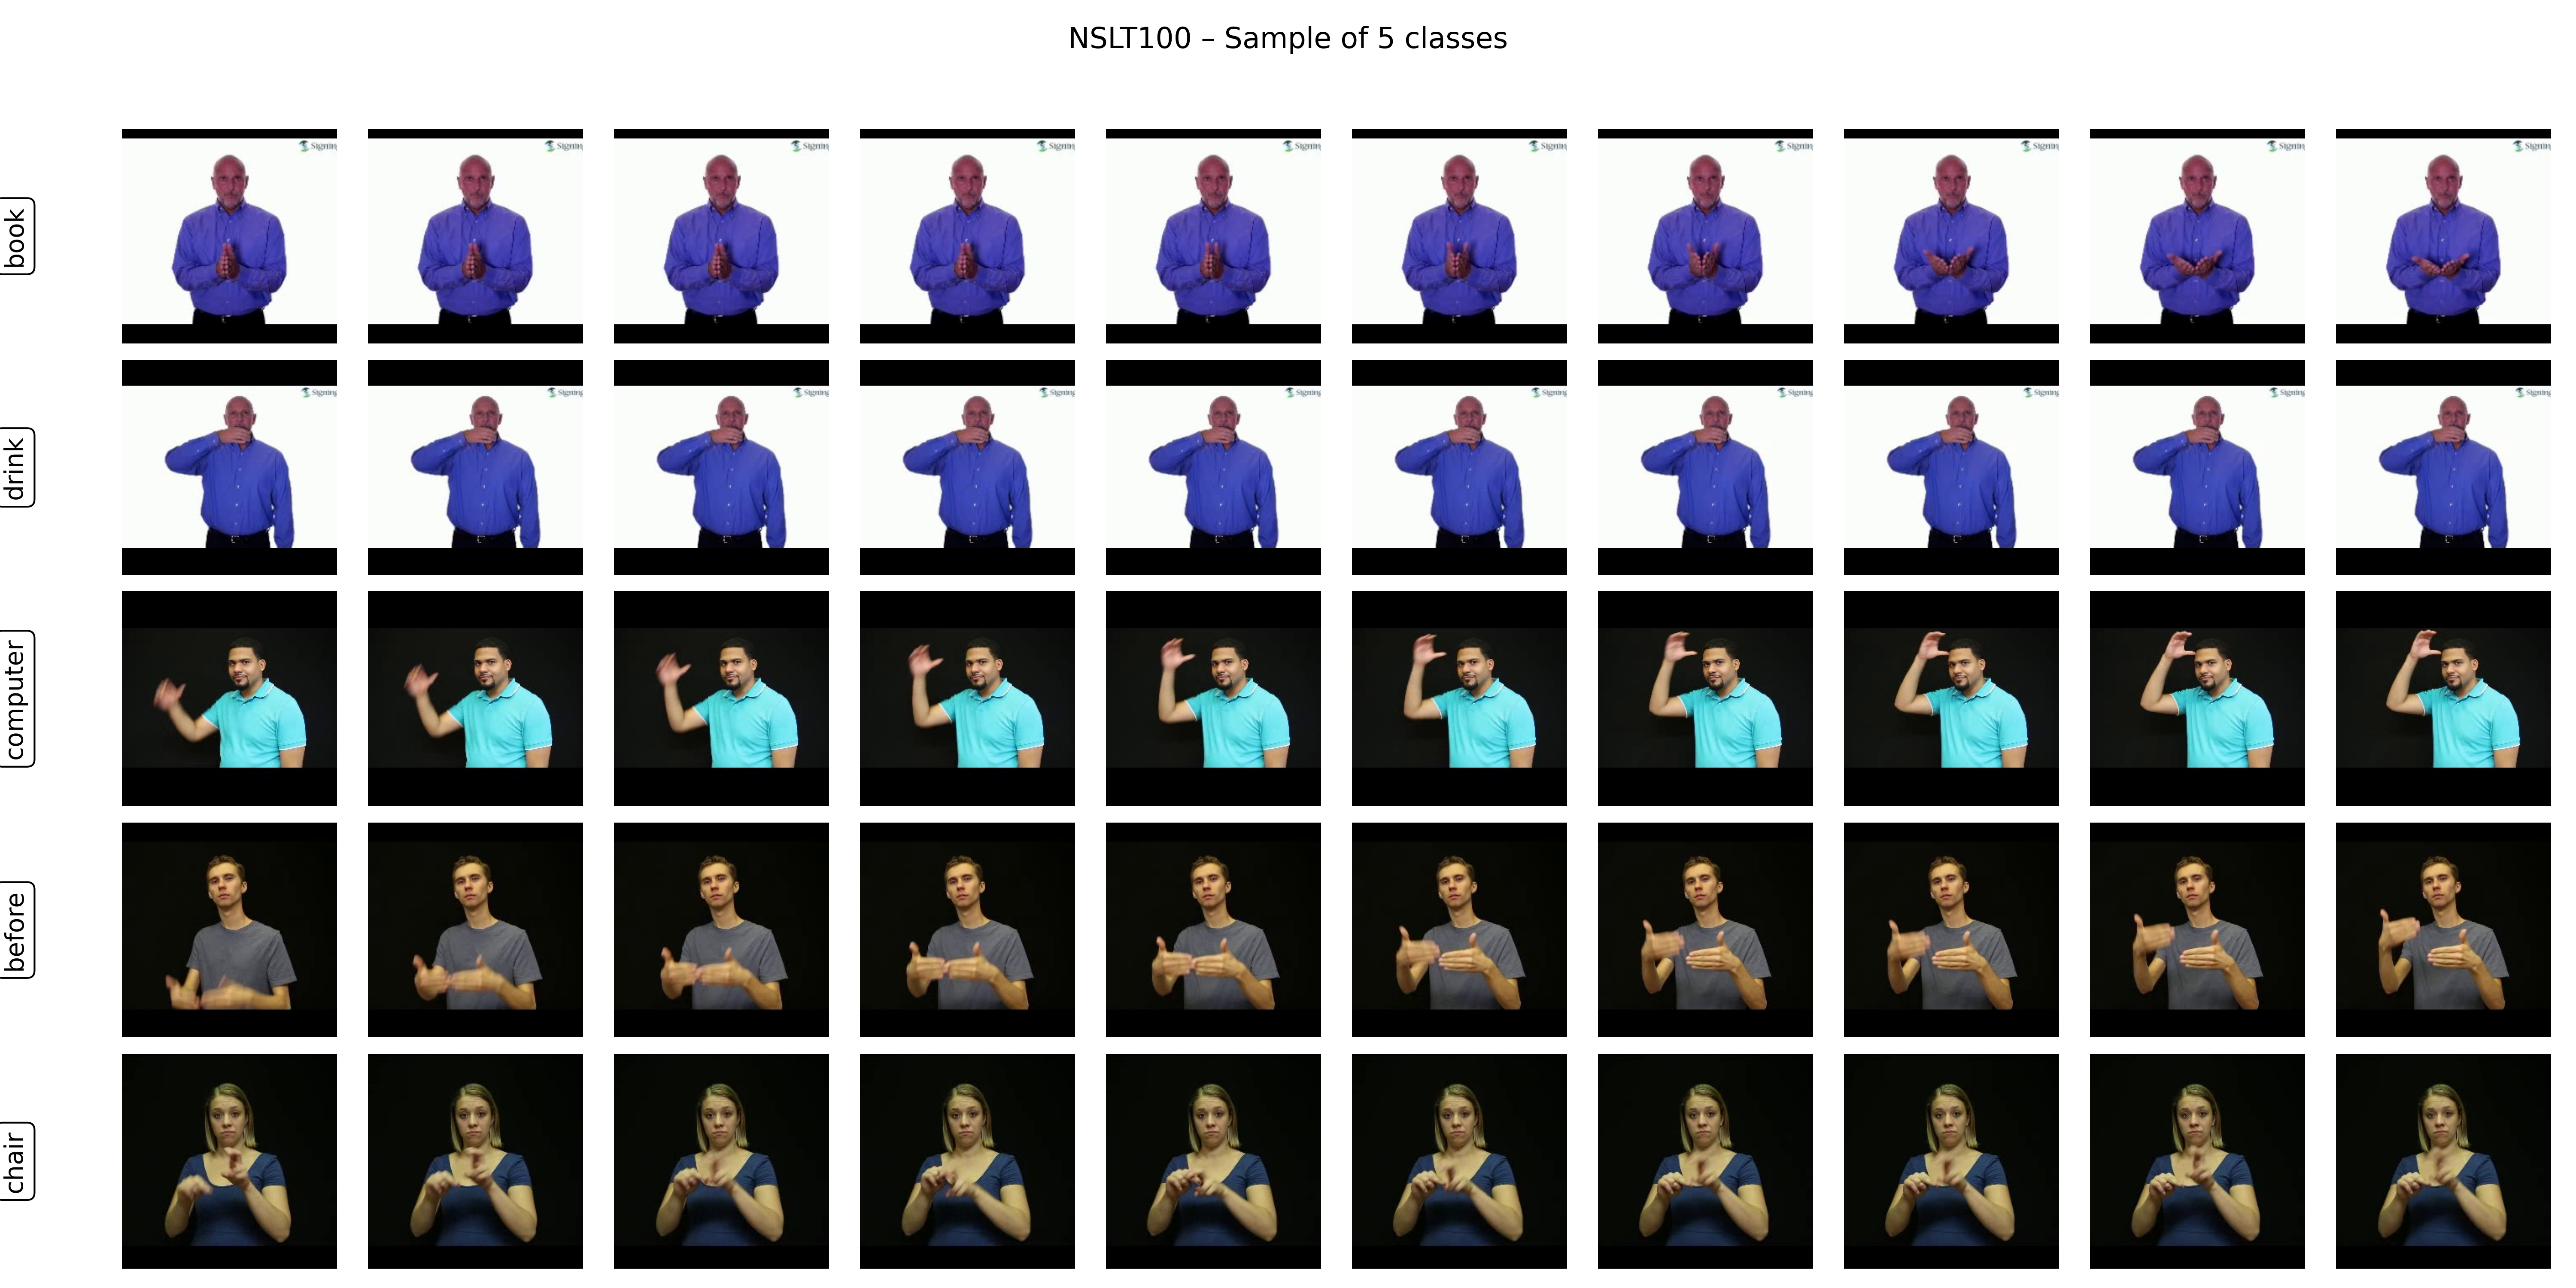
\includegraphics[width=1\linewidth]{Fig/nslt100_grid.png}
    \caption{Samples of NSLT100}
    \label{fig:nslt100}
\end{figure}

\subsection{Pre-processing}
Since the input data consists of raw videos, it must be pre-processed before being passed into the input layer of the model. This pre-processing phase includes two main stages: frame generation and landmark extraction.

\subsubsection{Frame Generation}
The first step of the pre-processing pipeline is the \textbf{Frame Generation}, which involves converting raw video into a fixed-length sequence of frames. This method is crucial for standardizing input dimensions for the model to read.

\vspace{0.5cm}

\noindent The frame generation process follows these steps:
\begin{enumerate}
  \item \textbf{Video Loading:} In the first step, I use OpenCV to read raw videos thanks to its a wide range of codecs and provides frame-level access to video content
  
  \item \textbf{Frame Extraction:} In this phase, the fixed length of frames is set by $T = 64$. For videos that have more frames than $T$, they will be calculated to adjust the amount of frames to 64 frames; for example, if a video has 120 frames, the frame step will be 2 and takes frames every 2 steps. In case of videos that have fewer frames than $T$, they will be padded by upsampling random frames except for the first and the last frame.
  
  \item \textbf{Frame Resizing and Normalization:} Each extracted frame is resized to a $H_v \times W_v$ with $H_v=W_v=224$, and normalized using the mean and standard deviation values expected by the pre-trained backbone model (S3D \cite{xie2017rethinking}). This step ensures compatibility with model input expectations and accelerates convergence during training.
\end{enumerate}

After this pre-processing stage, I obtain a fixed-size video tensor $\mathbf{V}$ with $\mathbf{V} \in \mathbb{R_V}^{T \times H_v \times W_v \times C}$, where $T = 64$ is the number of uniformly sampled frames, $H_v = W _v= 224$ are the spatial dimensions after resizing, and $C = 3$ represents the RGB color channels. 

\begin{figure}[H]
    \centering
    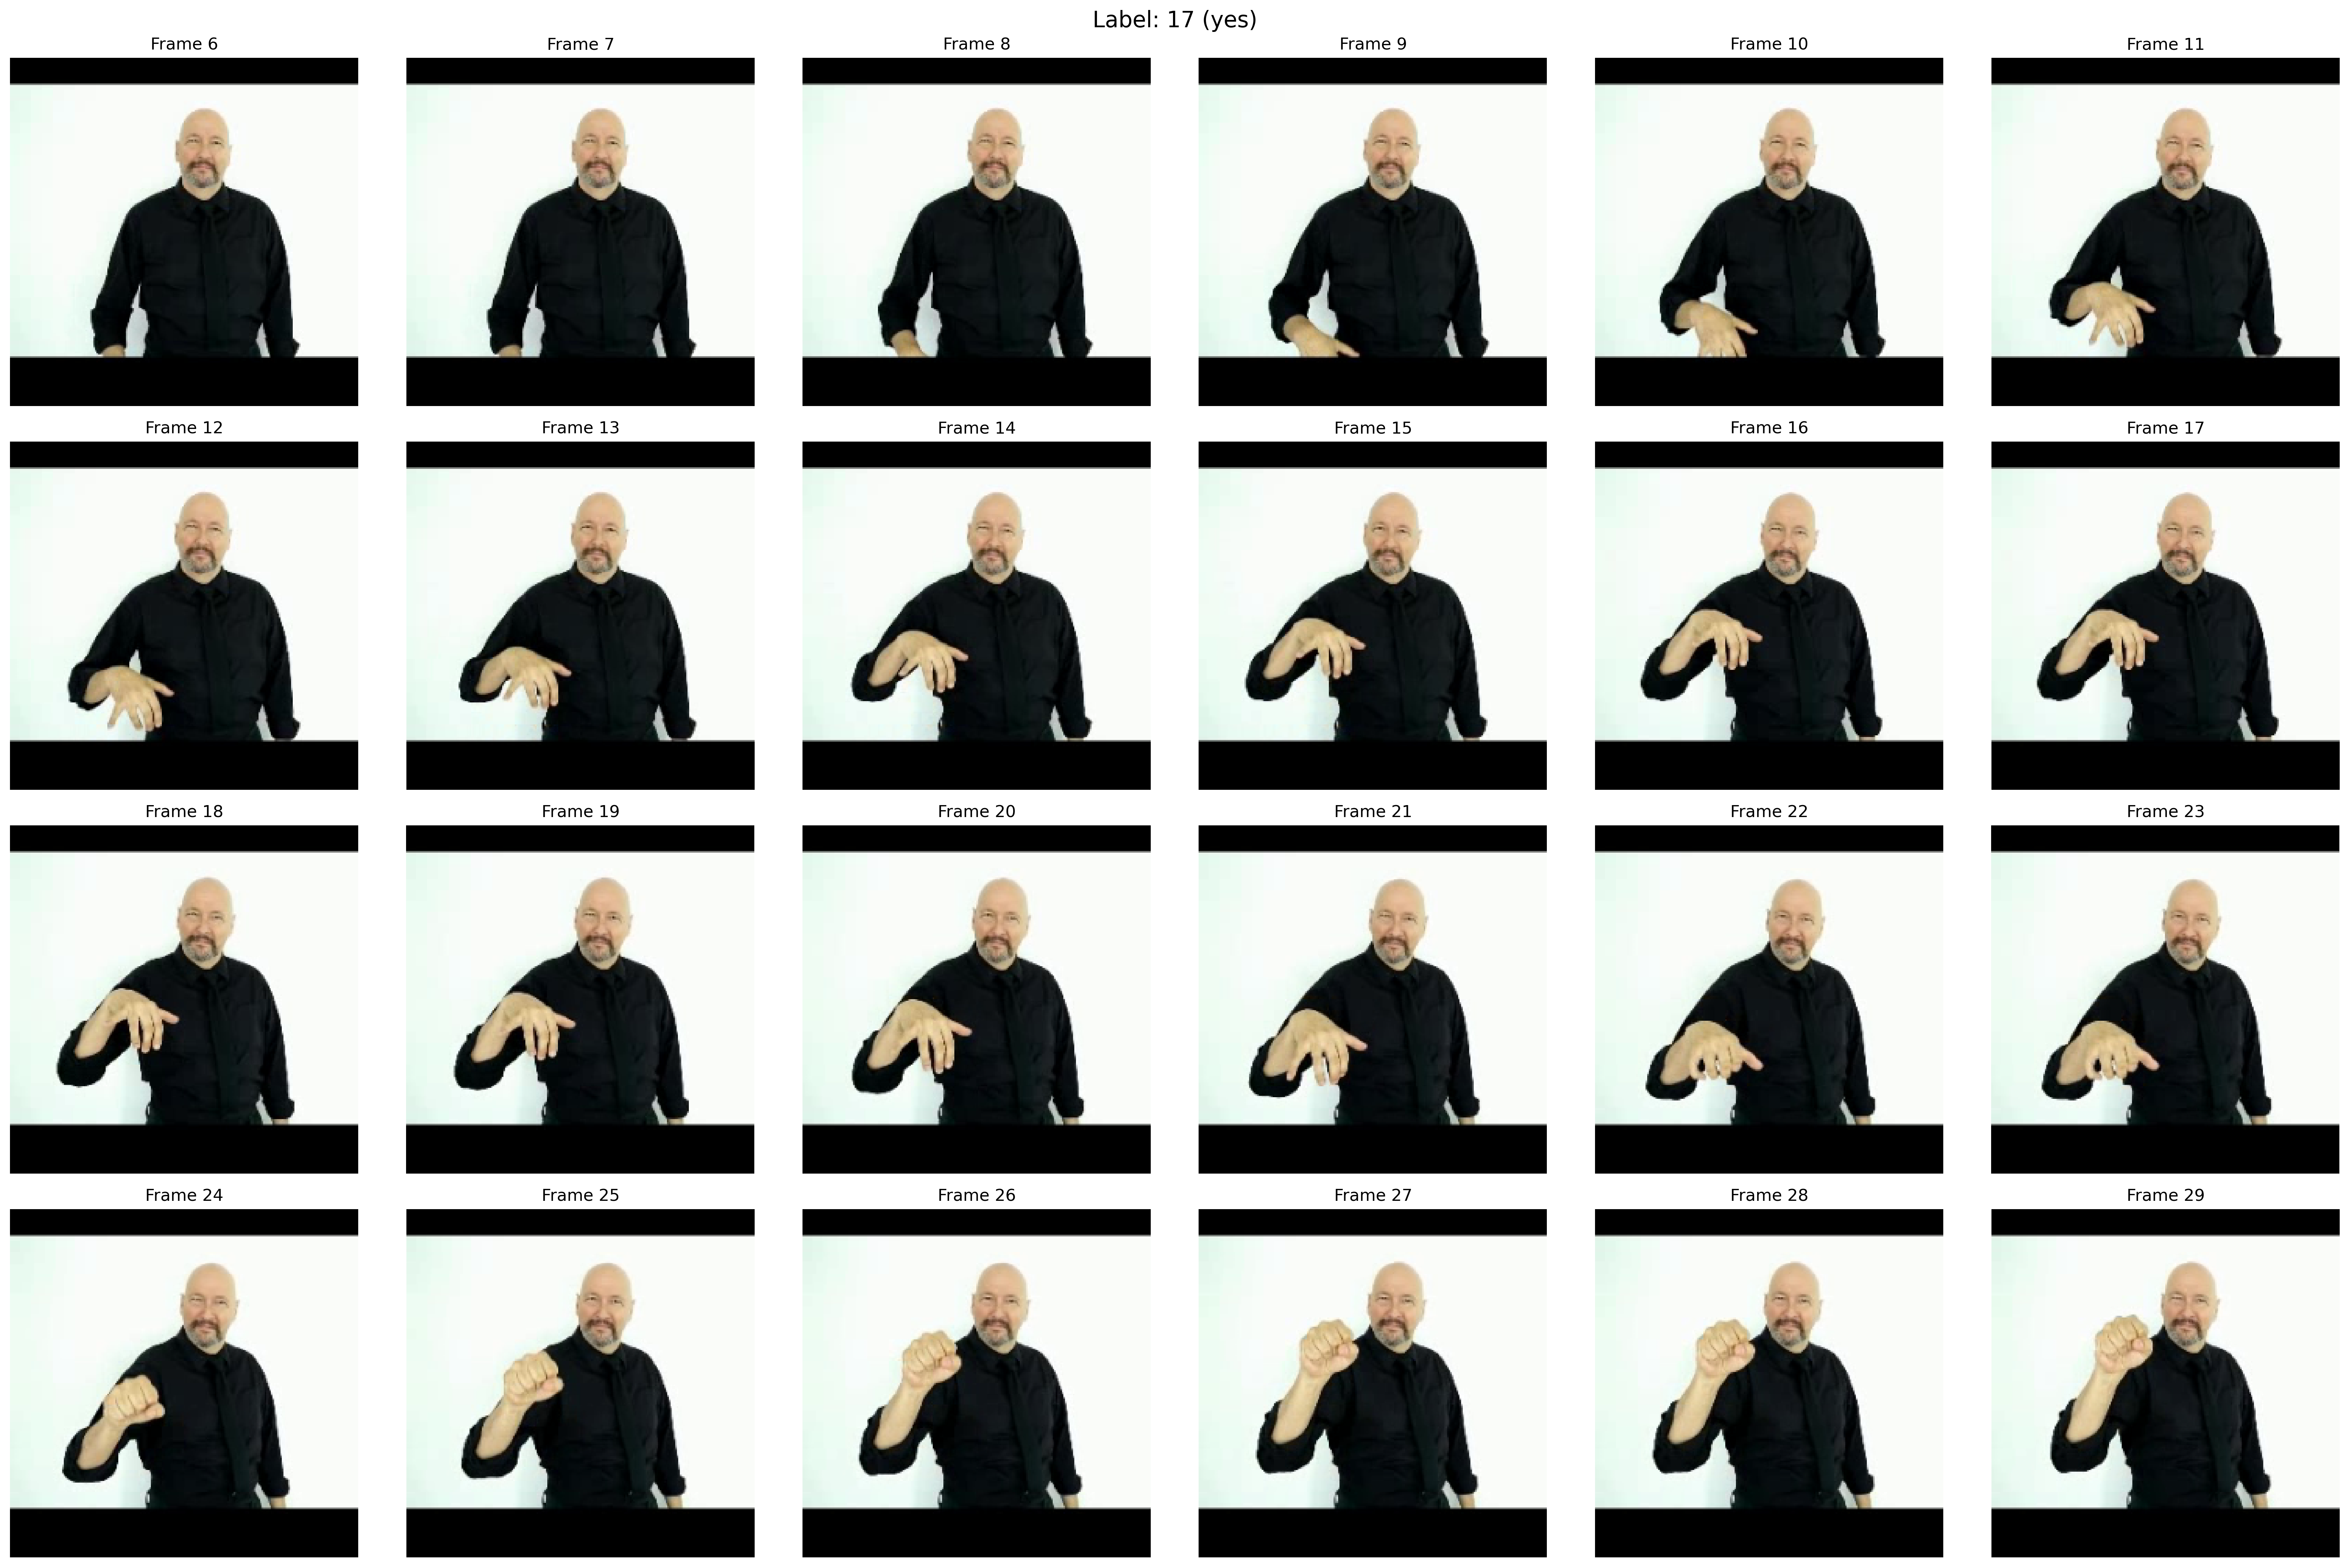
\includegraphics[width=1\linewidth]{Fig/64-frame.png}
    \caption{Example of Frame Generation}
    \label{fig:frame}
\end{figure}

\subsubsection{Landmark Extraction}
The second stage of the pre-processing pipeline is the \textbf{Landmark Extraction}, which involves extracting landmarks of body, face, and 2 hands. This method is important for the model to learn the temporal feature based on the movement and shifting of landmarks across the video frame sequence. In this part, I opt for Google Mediapipe \cite{mediapipe_holistic_landmarker} due to its accuracy and stable performance compared to other tools to extract landmarks such as VKNet \cite{zuo2023natural} based on HRNet \cite{sun2019deep} used in NLA-SLR \cite{zuo2023natural}.

\begin{figure}[H]
    \centering
    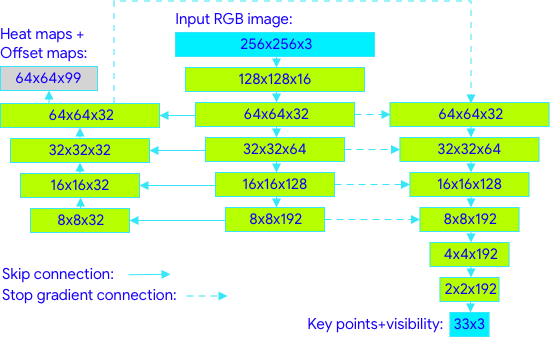
\includegraphics[width=0.85\linewidth]{Fig/PoseTrackerNet.png}
    \caption{Mediapipe (Blaze Model) Model on Pose}
    \label{fig:posemodel}
\end{figure}

\begin{table}[H]
\centering
\renewcommand{\arraystretch}{1.4}
\begin{tabular}{|>{\bfseries}l|p{5cm}|p{5cm}|}
\hline
\textbf{Aspect} & \textbf{MediaPipe (Blaze Models \cite{bazarevsky2020blazepose})} & \textbf{VKNet (HRNet-based \cite{sun2019deep})} \\
\hline
\textbf{Model Type} & Lightweight (3.5M \#Params, 6.9MFlops) & Heavyweight, high-capacity architecture (63.6M \#Params, 32.9 GFLOPs)\\
\hline
\textbf{Backbone} & BlazeFace, BlazePose, BlazeHand (custom MobileNet variants) & HRNet + 3D CNN (I3D or S3D for video) \\
\hline
\textbf{Accuracy} & PCK@0.2 of 97.2\% on AR dataset & High (used for precise keypoint tasks) \\
\hline
\textbf{Runtime Performance} & Real-time on mobile/embedded devices & Real-time only on high-end GPUs \\
\hline
\textbf{Input Size} & Low-resolution inputs (e.g., 256×256) & High-resolution inputs (e.g., 384×384+) \\
\hline
\textbf{Output} & 33 pose + 21 hand + 468 face landmarks & 17-133+ body landmarks (depending on dataset) \\
\hline
\textbf{Inference Speed} & ~30–60 FPS on mobile/desktop & ~10–25 FPS (depending on hardware) \\
\hline
\textbf{Target Platform} & Mobile, Web, Edge devices & Desktop, Cloud, Research-grade GPUs \\
\hline
\textbf{Use Case} & AR filters, fitness apps, gesture tracking & Pose estimation, sign language recognition, motion capture \\
\hline
\end{tabular}
\caption{Comparison between MediaPipe Blaze models and VKNet (HRNet-based) for landmark detection}
\end{table}

After the above comparison, Google Mediapipe is believed to be lighter and still maintains accuracy when used for the landmark extracting task. In this case, I selected a holistic model, which is a combination of pose model, hand model and face mesh model. It yields 543 keypoints in total with 33 keypoints for pose, 21 keypoints per hand and 468 keypoints for face in three dimensions $x, y, z$.

\begin{figure}[htpb]
    \centering
    \begin{minipage}[b]{0.32\textwidth}
        \centering
        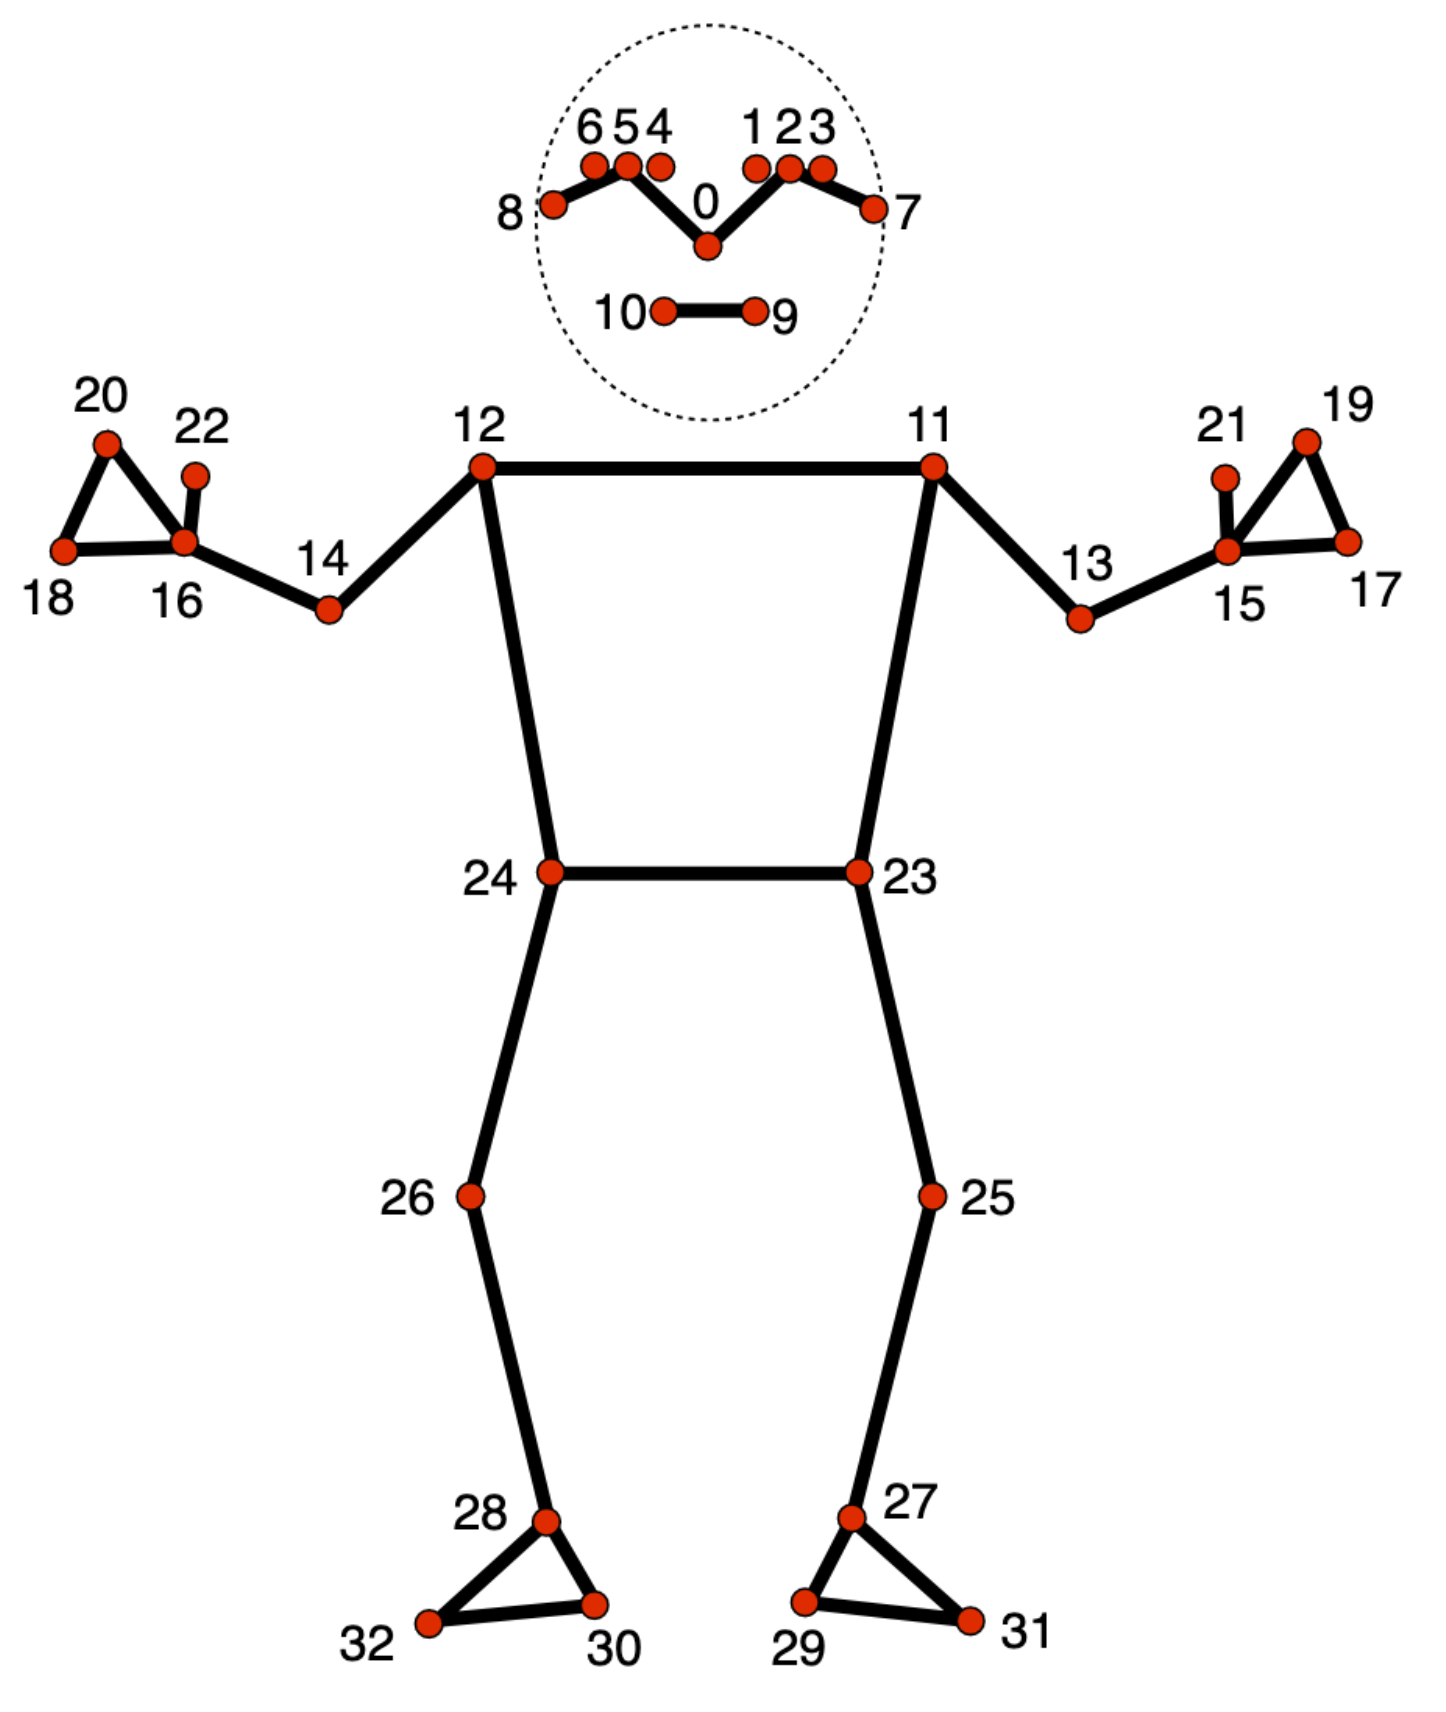
\includegraphics[width=0.75\linewidth]{Fig/pose_landmarks_index.png}
        \caption{(a) Pose Landmark}
    \end{minipage}
    \hspace{1cm}
    \begin{minipage}[b]{0.32\textwidth}
        \centering
        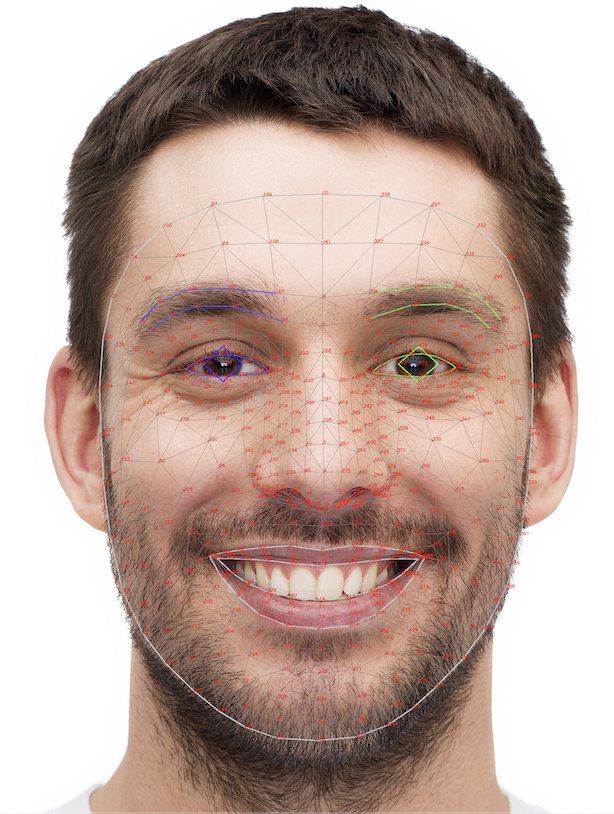
\includegraphics[width=0.75\linewidth]{Fig/face_landmarker_keypoints.png}
        \caption{(b) Face Landmark}
    \end{minipage}
    \label{fig:mediapipe1}
\end{figure}

\begin{figure}[H]
    \centering
    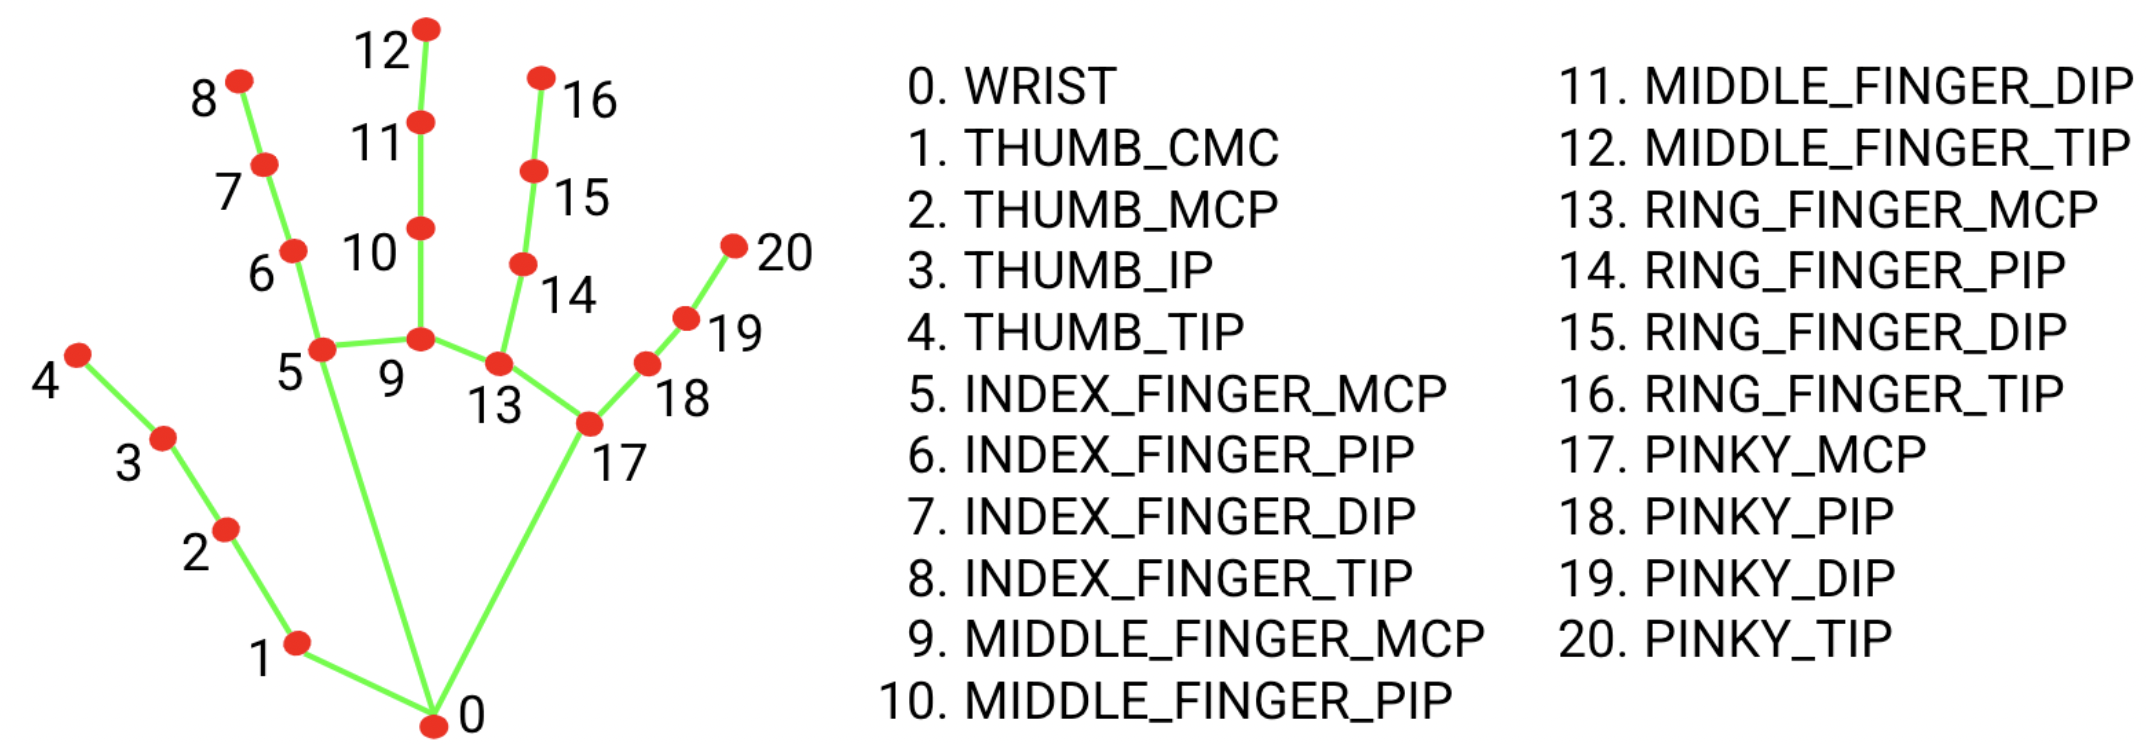
\includegraphics[width=1\linewidth]{Fig/hand-landmarks.png}
    \caption{(c) Hand Landmark}
    \label{fig:mediapipe2}
\end{figure}

After this pre-processing stage, I receive a fixed-size landmark tensor $\mathbf{L}$ with $\mathbf{L} \in \mathbb{R_L}^{T \times N \times D}$, where $T = 64$ is the number of uniformly sampled frames, $N$ is the number of landmarks, and $D = 3$ represents the dimension of extracted landmarks.

\begin{figure}[H]
    \centering
    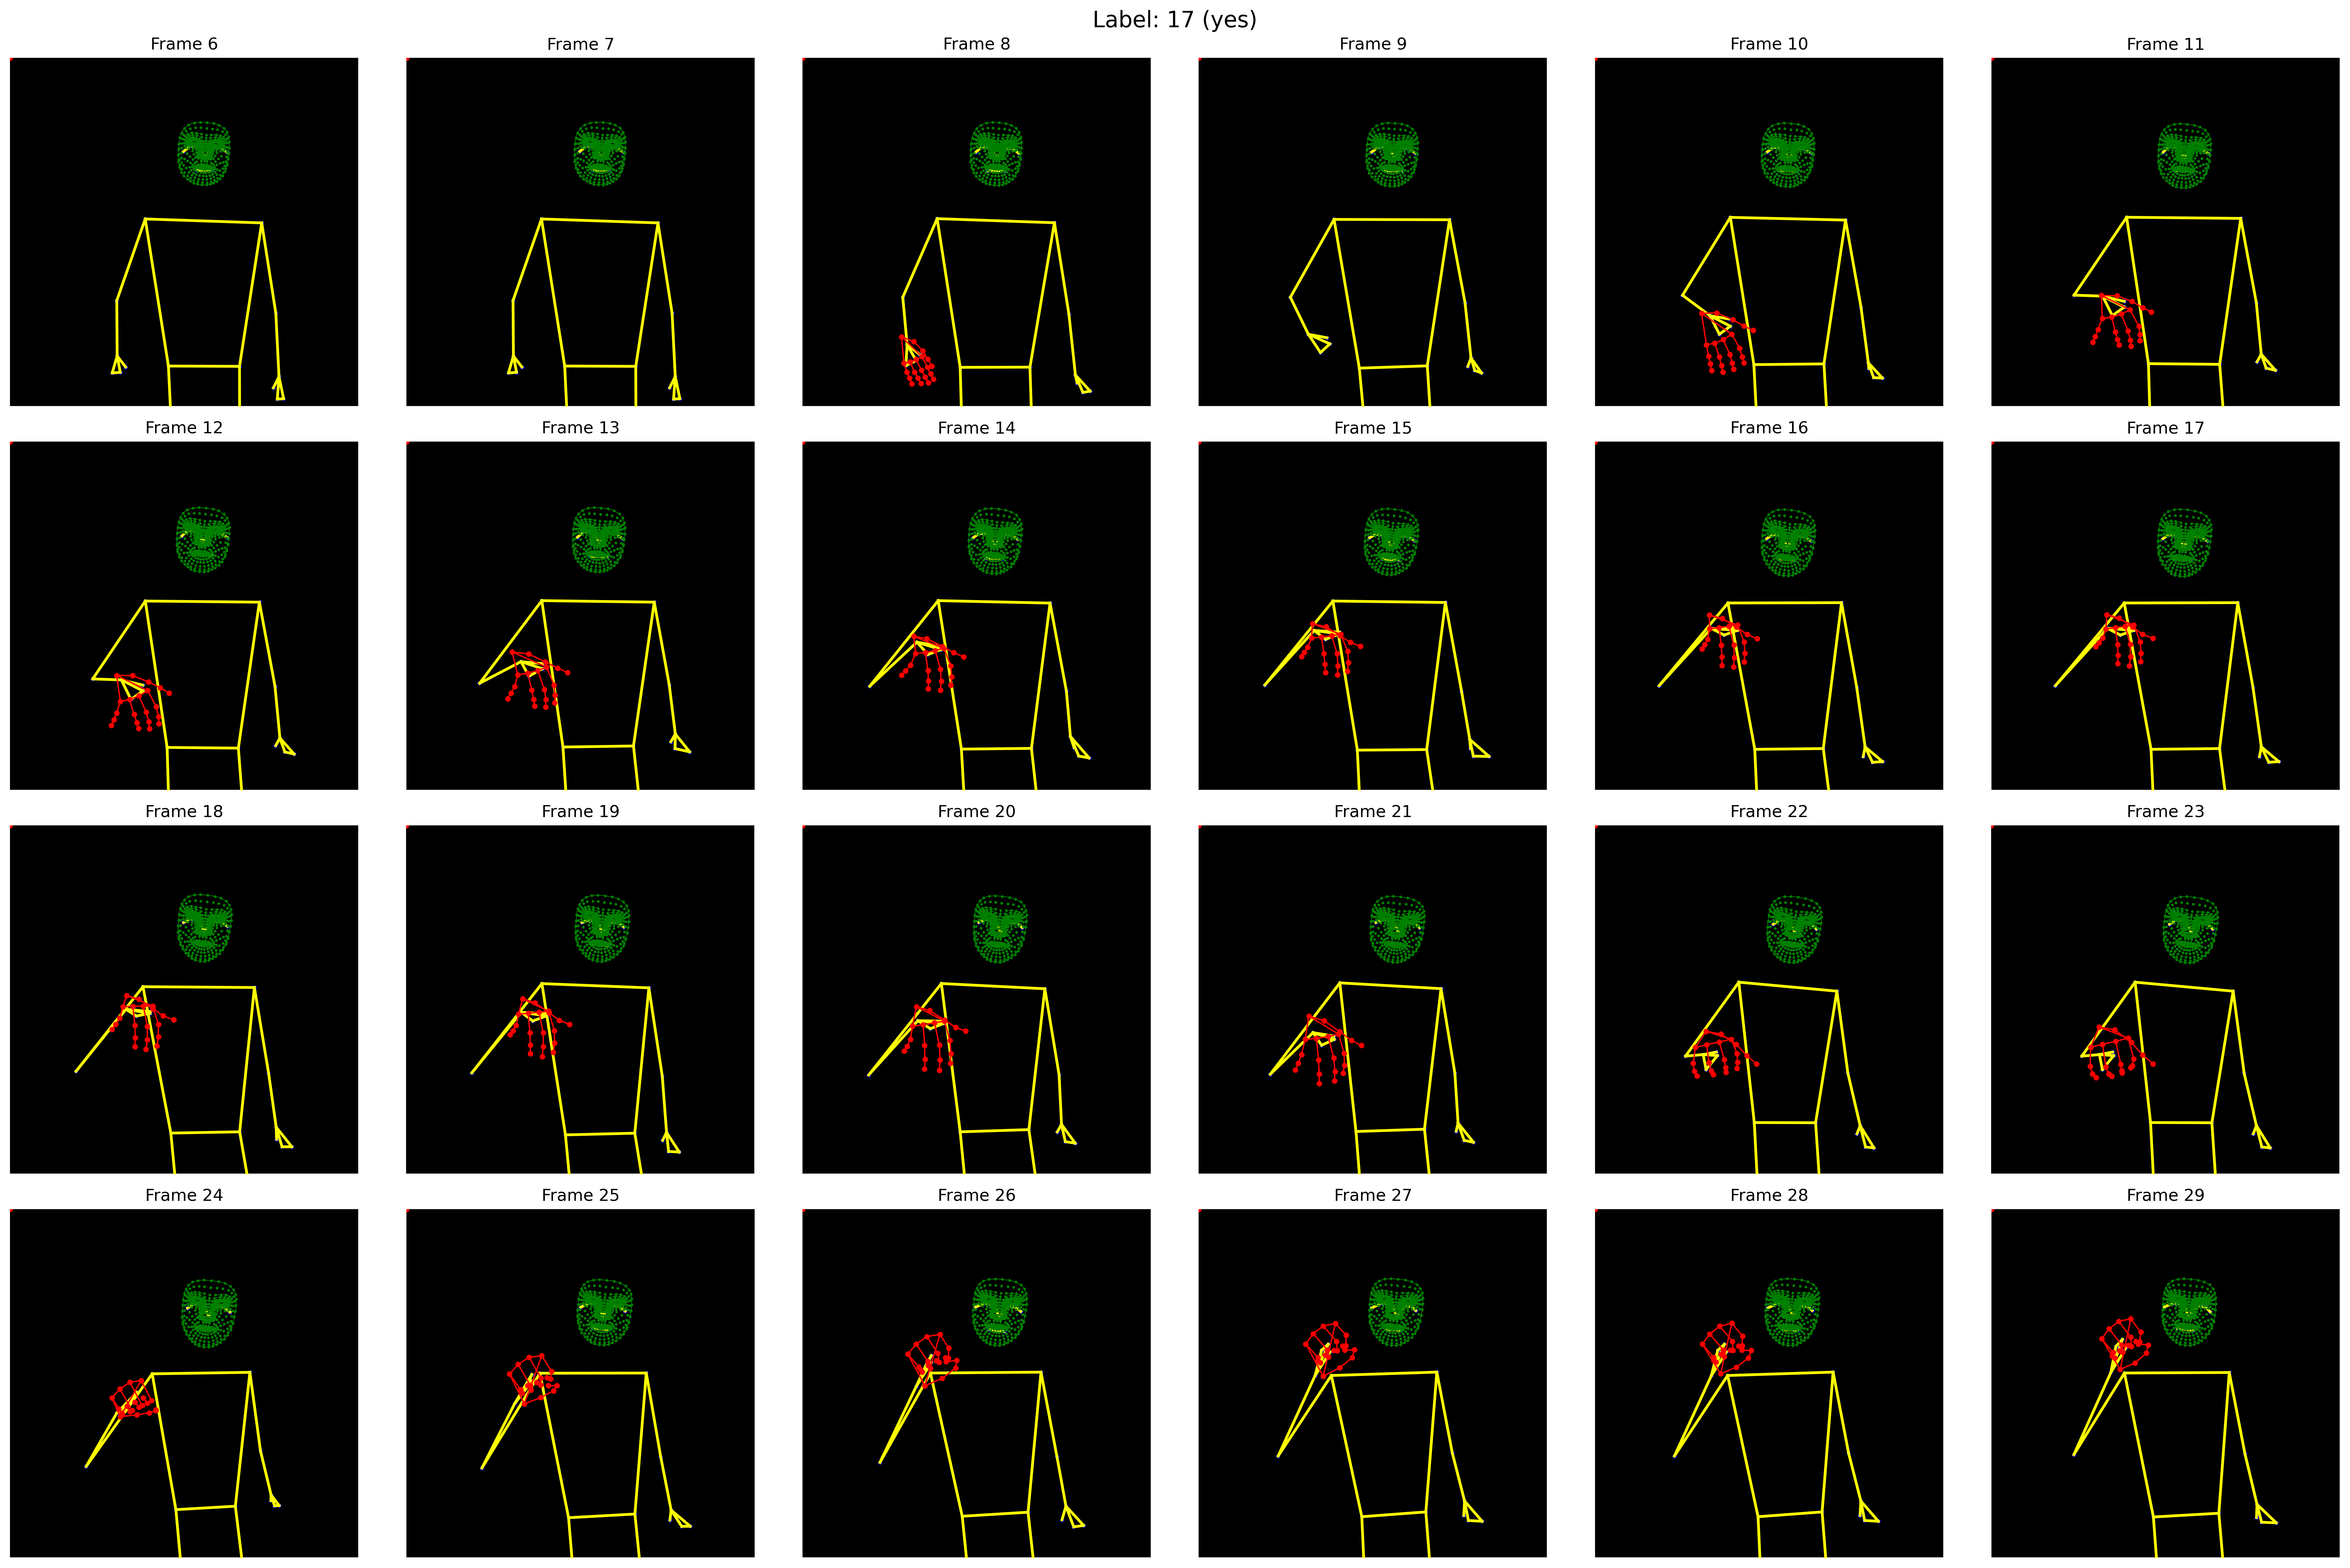
\includegraphics[width=0.95\linewidth]{Fig/64-landmarks.png}
    \caption{Extracted Landmarks}
    \label{fig:landmark-draw}
\end{figure}

\begin{figure}[H]
    \centering
    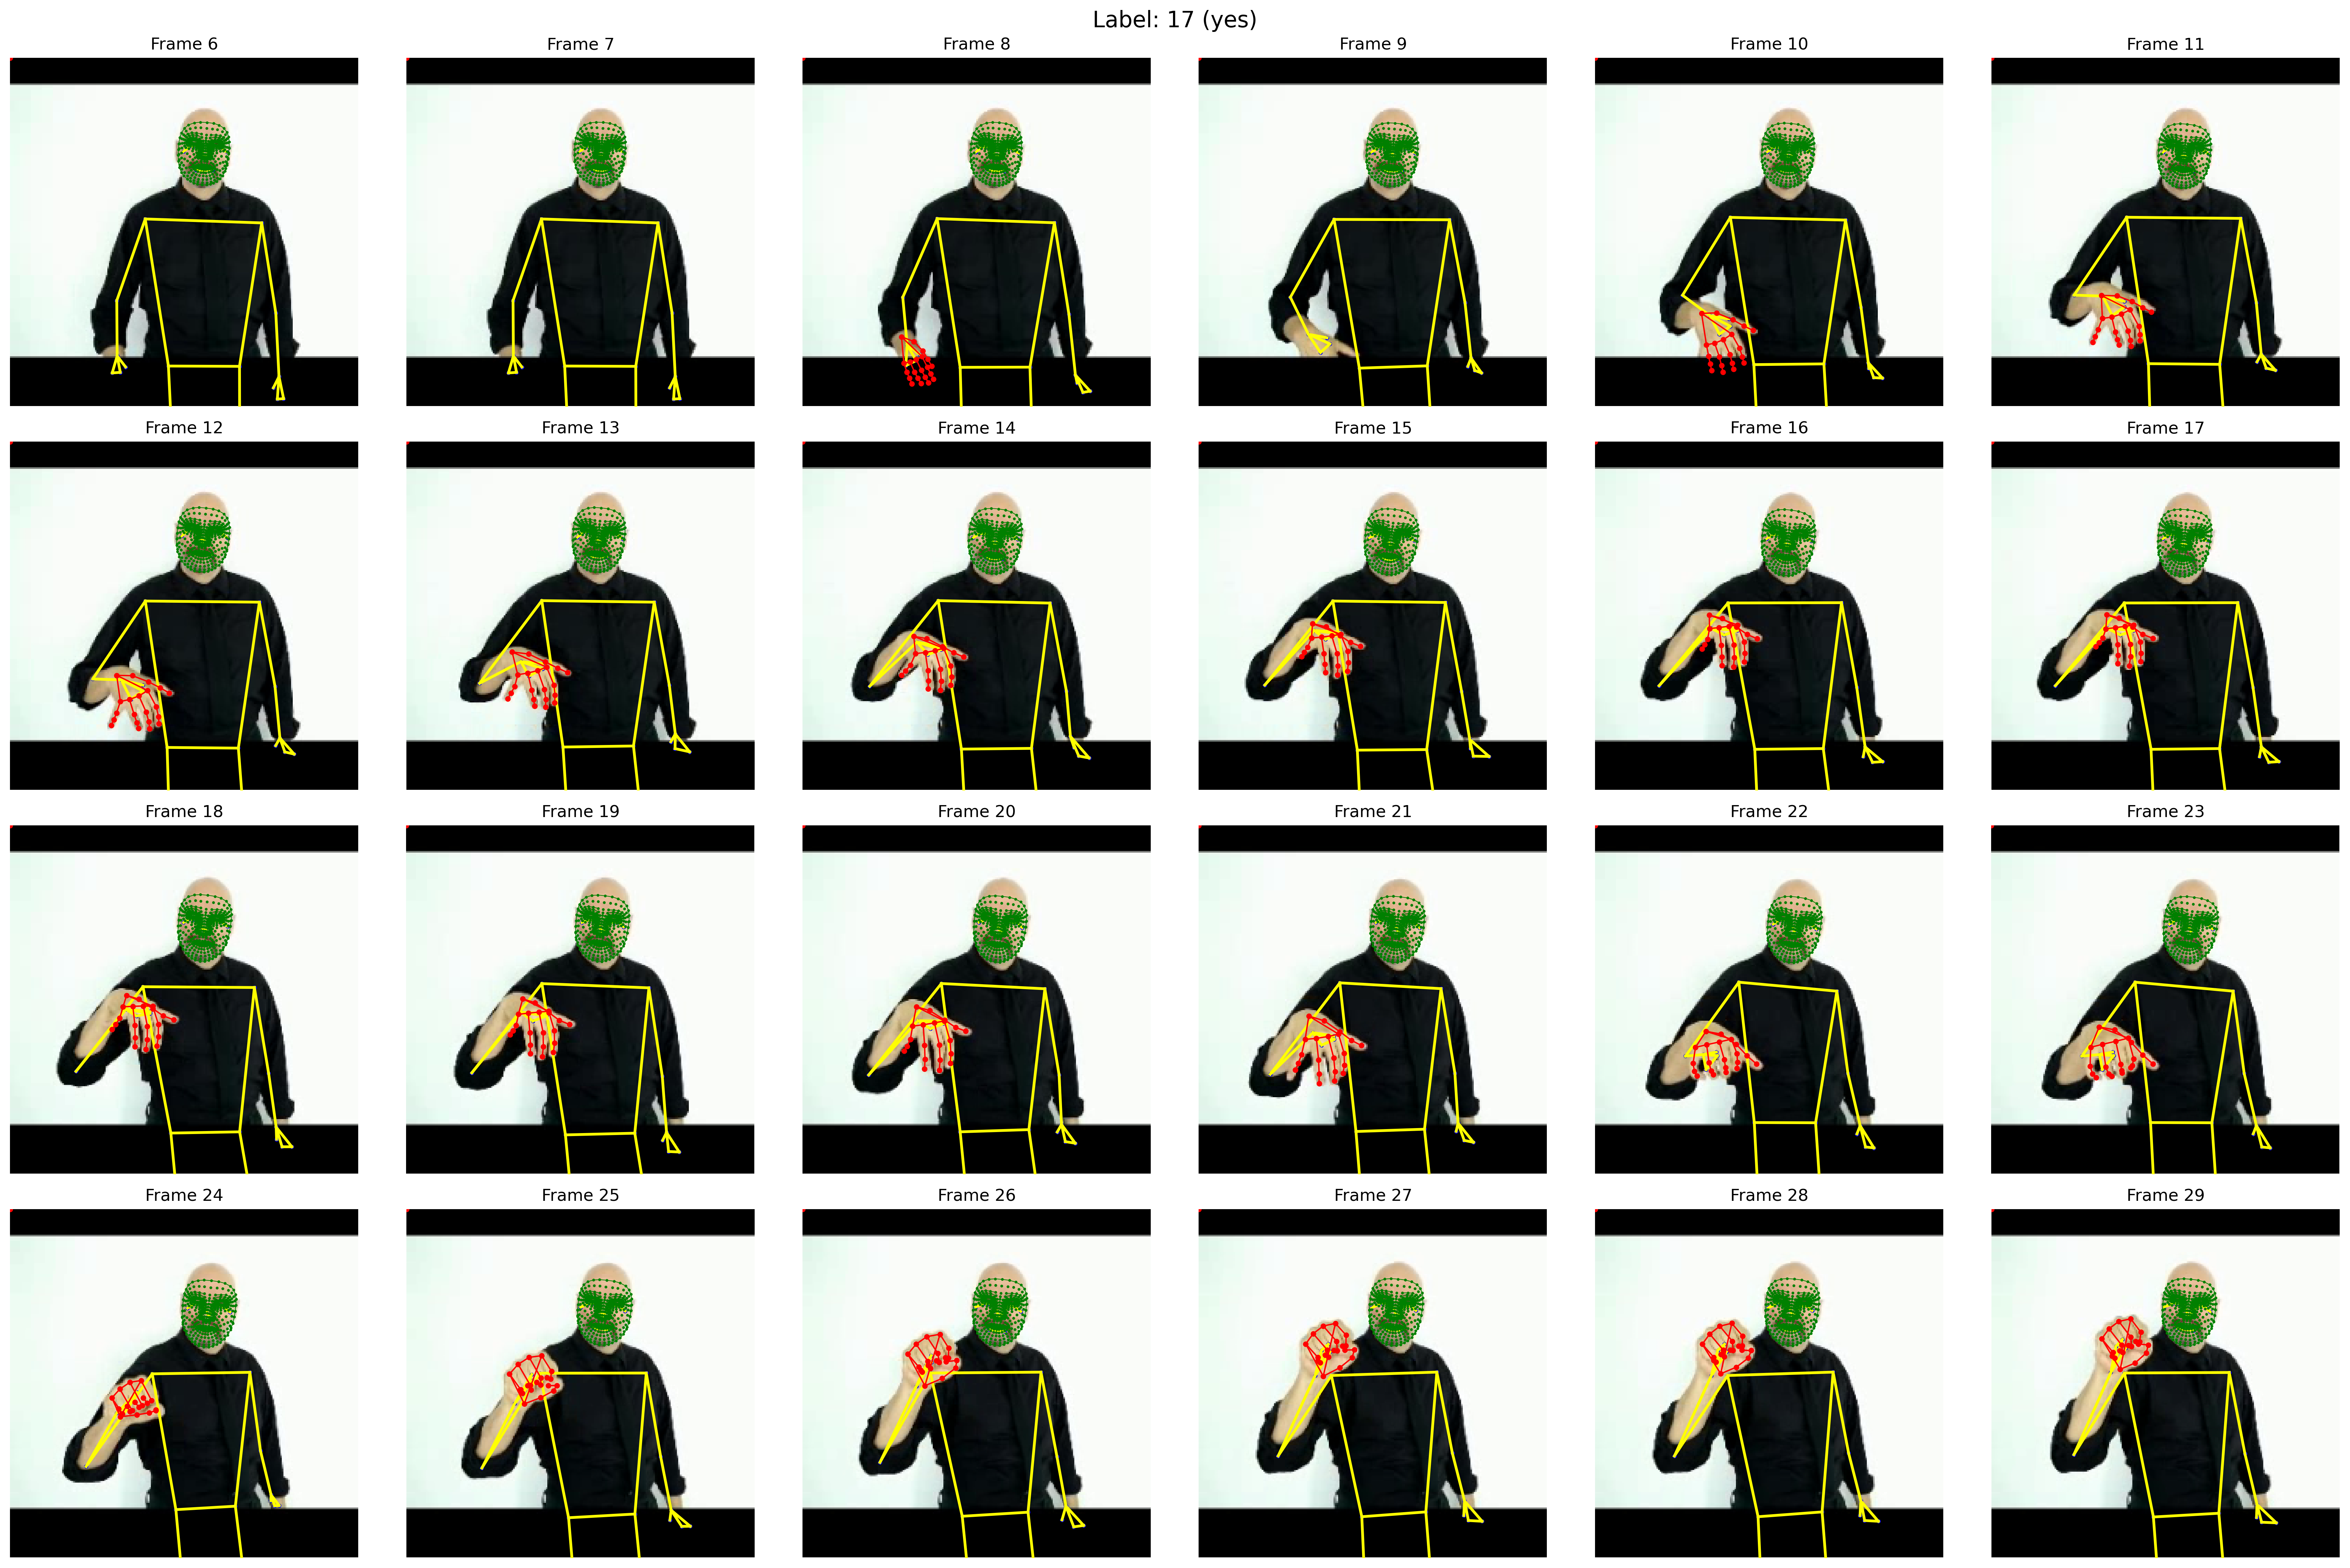
\includegraphics[width=0.95\linewidth]{Fig/64-frame-landmarks.png}
    \caption{Extracted Landmarks on Frames}
    \label{fig:framelandmark}
\end{figure}

\subsubsection{Combined Data}
In the next step, the video tensors and landmark tensors are combined and returned in a unified dictionary format $\mathbf{Data}$, along with the corresponding label, a binary mask indicating valid frames, and the video path that $\mathbf{Data} \in \mathbb{R}^{\mathbb{R_V} \times \mathbb{R_L} \times Label \times Mask}$ where $\mathbb{R_V}$ represents video tensor and $\mathbb{R_L}$ is landmark tensor. And finally, I batch the $\mathbf{Data}$ with batch size of 8 and partition it into train, validation and test set corresponding to the split in the official NSLT100.

\begin{table}[h]
\centering
\renewcommand{\arraystretch}{1.3}
\begin{tabular}{|>{\bfseries}l|l|}
\hline
\textbf{Key} & \textbf{Tensor Shape} \\
\hline
\texttt{video} & \texttt{[8, 3, 64, 224, 224]} \\
\hline
\texttt{landmarks} & \texttt{[8, 64, 543, 3]} \\
\hline
\texttt{mask} & \texttt{[8, 64]} \\
\hline
\texttt{label} & \texttt{[8]} \\
\hline
\texttt{video\_path} & List of strings (file paths) \\
\hline
\end{tabular}
\caption{Batch Dictionary Keys and Corresponding Tensor Shapes}
\end{table}

\subsection{Transfer Learning with SLN Model}
This section details my deep learning model for SLR, which uses the S3D backbone \cite{xie2017rethinking} with Landmark Transformer built based on STEPNET model \cite{pan2022stepnet}. The goal is to figure out the challenge of temporal features in a sequence of frames. S3D is used to address video-based features and Landmark Transformer is applied to focus on temporal features learned through landmark shifting, and they allow fuse model SLN to learn and recognize signs precisely. The integration aims to significantly boost classification accuracy and generalize well across diverse signs.

\subsubsection{S3D Model}

\begin{figure}[H]
    \centering
    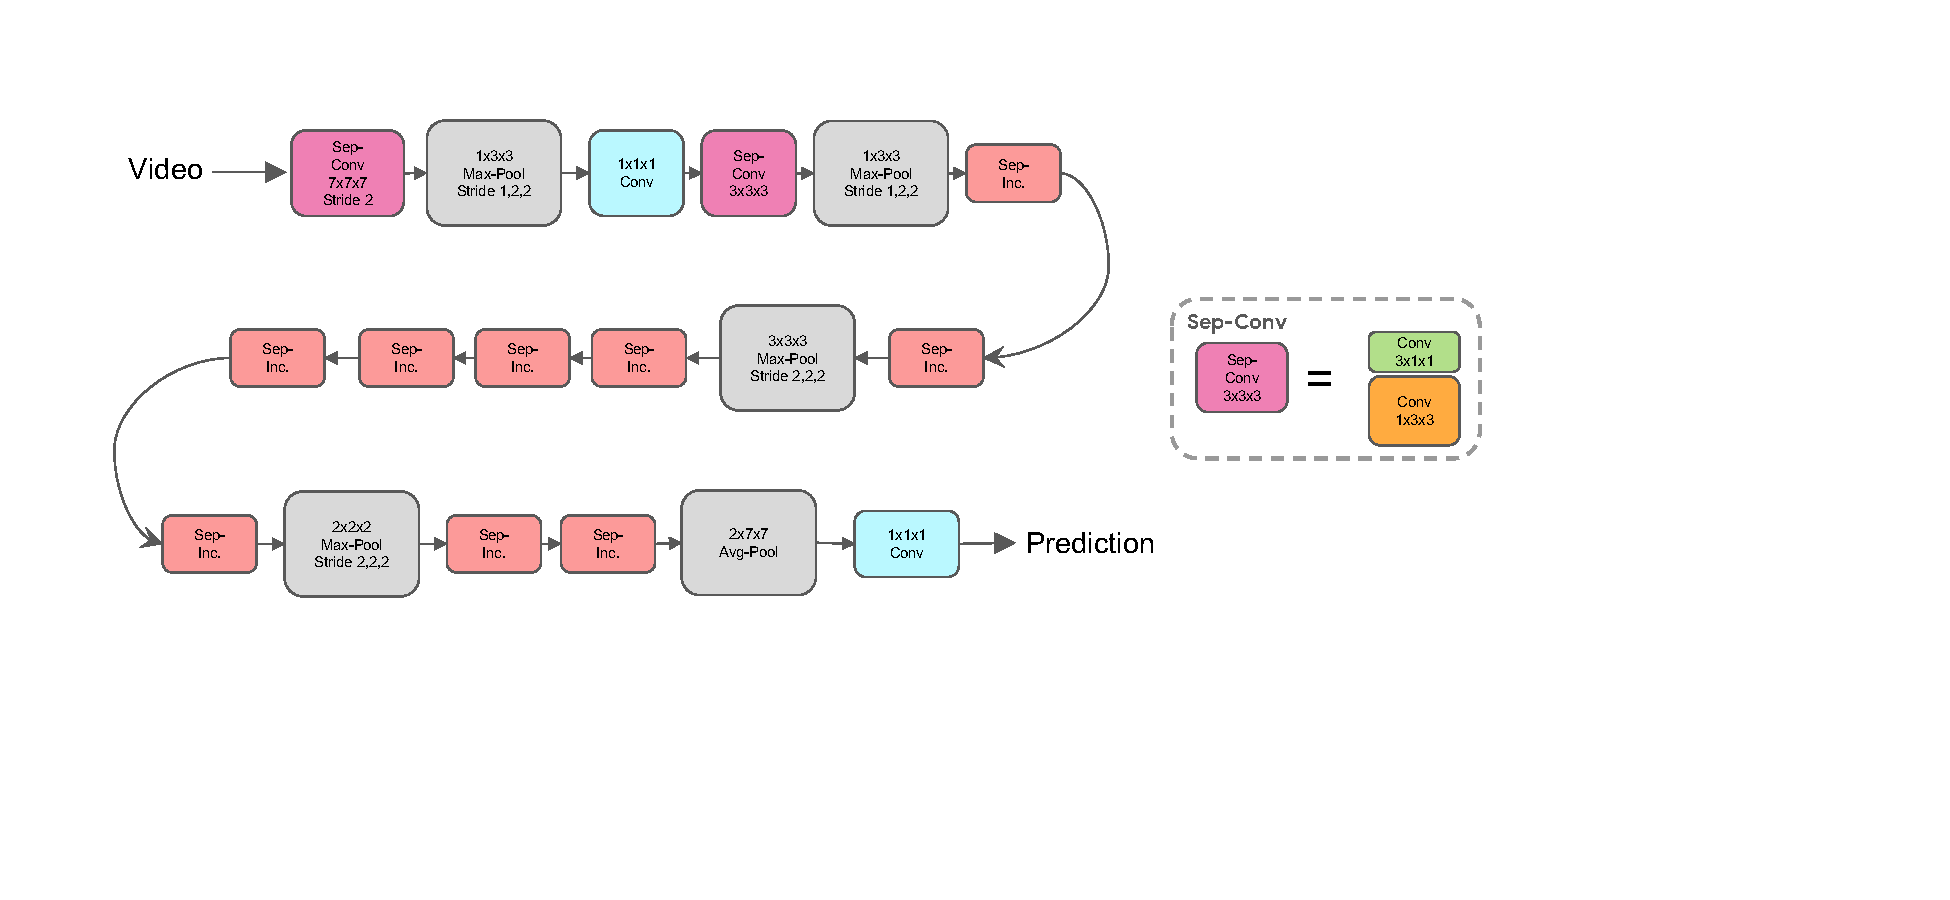
\includegraphics[width=1\linewidth]{Fig/s3dg.pdf}
    \caption{S3D Architecture}
    \label{fig:s3dmodel}
\end{figure}

The S3D (Separable 3D) convolutional network is a lightweight and efficient model applying spatiotemporal feature extraction from video data. In the model paper, it extends traditional 2D convolutional networks by extracting a temporal dimension and make it suitable for SLR.

\vspace{0.5cm}

S3D is built based on the Inception architecture and \textit{factorized 3D convolutions}, which significantly reduce computational complexity. Instead of applying a full 3D convolution over spatial and temporal dimensions simultaneously, S3D factorizes it into a 2D spatial convolution followed by a 1D temporal convolution. This method reduces the number of parameters and increases the speed of training while maintaining the model's ability to capture motion and appearance features effectively.

\vspace{0.5cm}

In this project, S3D serves as the primary video backbone. Pretrained weights (trained on the Kinetics-400 dataset \cite{kay2017kinetics}) are used to leverage general spatiotemporal patterns learned from large-scale video. Each input video is rearranged the shape from $[B, T, H, W, C]$ represented as a tensor of shape $[B, C, T, H, W]$, where $B$ is the batch size, $C = 3$ represents RGB channels, $T = 64$ is the number of frames, and $H = W = 224$ are the spatial dimensions. The classifier head of the original S3D network is removed and yields video-based feature maps $f_V$.

\subsubsection{Landmark Transformer}

\begin{figure}[H]
    \centering
    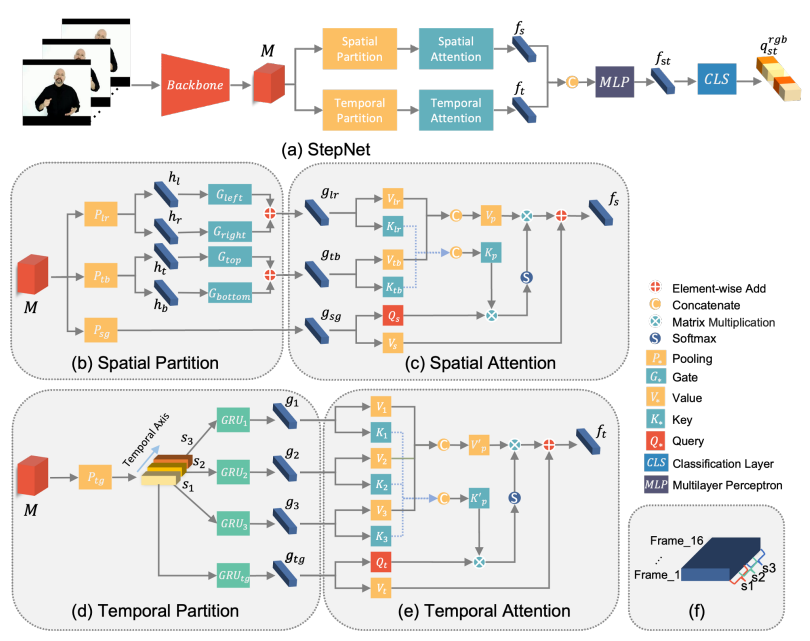
\includegraphics[width=1\linewidth]{Fig/stepnet.png}
    \caption{STEPNET Architecture}
    \label{fig:stepnetmodel}
\end{figure}

StepNet is a model designed to enhance SLR by capturing motion patterns from the body. It works by segmenting the hand movement sequence into overlapping temporal windows and applying attention-based encoding to extract dynamic features across time. In this project, I will fine-tune this model so that the SLN model can learn the pattern of landmark shifting across time.

\vspace{0.5cm}

To model the temporal dynamics of body landmarks in sign language recognition, a dedicated module called the \textbf{Landmark Transformer}, inspired by the StepNet architecture, is employed. This module extracts motion-aware features from 3D landmark sequences representing the face, pose, and both hands.

\subsubsubsection{Spatial Partitioning}
The input landmark tensor of shape $[B, T, 543, 3]$ is partitioned into four semantically distinct regions:
\begin{itemize}
    \item \textbf{Pose} $K^{pose} \in \mathbb{R}^{B \times T \times 33 \times 3}$: 33 keypoints ($0$–$32$)
    \item \textbf{Face} $K^{face} \in \mathbb{R}^{B \times T \times 468 \times 3}$: 468 keypoints ($33$–$499$)
    \item \textbf{Left Hand} $K^{left} \in \mathbb{R}^{B \times T \times 21 \times 3}$: 21 keypoints ($500$–$521$)
    \item \textbf{Right Hand} $K^{right} \in \mathbb{R}^{B \times T \times 21 \times 3}$: 21 keypoints ($522$–$543$)
\end{itemize}
This separation enables the model to learn localized attention within each region independently.

\subsubsubsection{Spatial Attention}
Each group of landmarks is passed through a shared spatial attention mechanism that computes a context-aware representation for each frame. This is achieved using self-attention with queries, keys, and values derived from linear projections of the input. The attention output is averaged over the landmark dimension to obtain a feature tensor of shape $[B, T, D]$ for each region.Each region is processed using a shared self-attention mechanism to learn spatially aware embeddings per frame. For a region $R \in \mathbb{R}^{B \times T \times N \times D}$:
\[
Q = RW_Q, \quad K = RW_K, \quad V = RW_V
\]
\[
\text{Attn}(R) = \text{softmax} \left( \frac{QK^\top}{\sqrt{d}} \right)V, \quad f^{R} = \frac{1}{N} \sum_{i=1}^{N} \text{Attn}(R_i)
\]
The outputs $f^{pose}$, $f^{left}$, $f^{right}$, and $f^{face}$ are then summed:
\[
f_{spatial} = f^{pose} + f^{left} + f^{right} + f^{face} \in \mathbb{R}^{B \times T \times d}
\]

\subsubsubsection{Temporal Partitioning}
To better capture local motion patterns, the combined spatial features are partitioned into overlapping temporal windows. If the temporal length is $T$, a window size $W$ and overlap $O$ are used to generate multiple segments, resulting in a tensor of shape $[B, S, W, D]$, where $S$ is the number of segments.The temporal dimension is segmented into overlapping windows:
\[
S_j = f_{spatial}[:, j:j+W, :] \quad \text{for } j = 0, \Delta, 2\Delta, \dots
\]
producing $S \in \mathbb{R}^{B \times N_s \times W \times d}$, where $W$ is the window size and $\Delta = W - \text{overlap}$.

\subsubsubsection{Temporal Attention with BiGRU}
Each temporal segment is processed by a bidirectional GRU, and the hidden states are aggregated using an attention mechanism to produce a weighted representation of important temporal patterns. Each segment $S_j$ is passed through a BiGRU to extract temporal patterns. Let $h_j = \text{BiGRU}(S_j) \in \mathbb{R}^{B \times 2H}$. The final segment-level representation is computed using attention:
\[
\alpha_j = \text{softmax}(W_2 \tanh(W_1 h_j)), \quad f_{temporal} = \sum_{j=1}^{N_s} \alpha_j h_j
\]
The result is a motion-aware embedding $f_K \in \mathbb{R}^{B \times 2H}$, representing the temporal evolution of body landmarks.

\subsubsubsection{Final Output}
The final temporal attention output serves as a representation of the landmark sequence feature $f_K$ and is later fused with video-based features for final classification. This method enhances the model's ability to capture both visual and kinematic aspects of sign language. 

\begin{figure}[H]
    \centering
    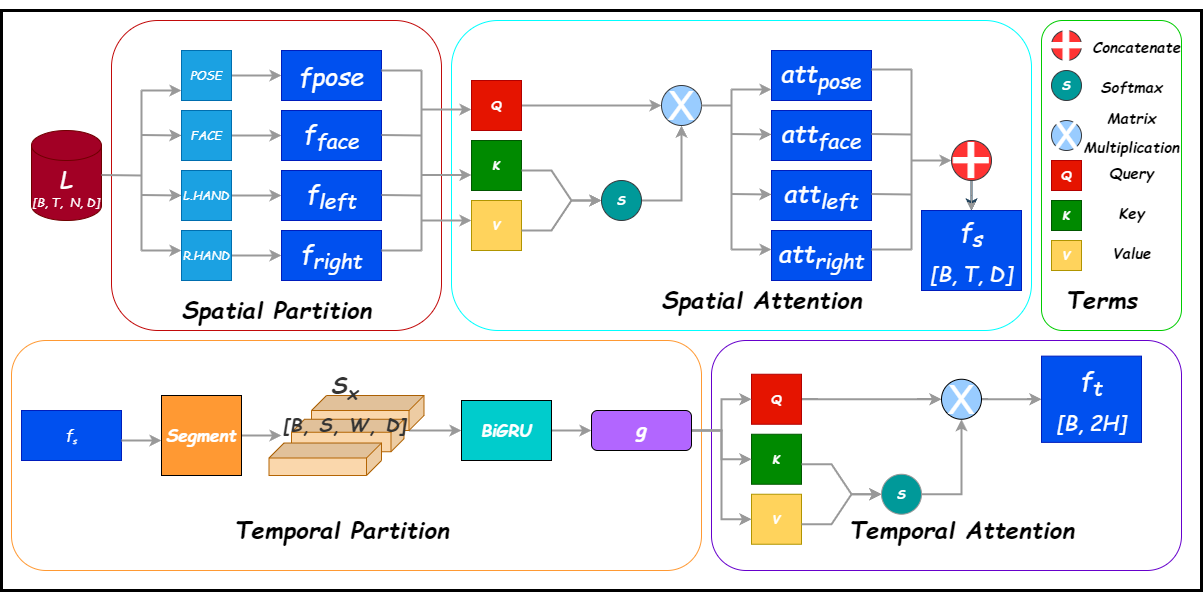
\includegraphics[width=0.9\linewidth]{Fig/LandMarks.drawio.png}
    \caption{Landmark Transformer Architecture}
    \label{fig:landmark}
\end{figure}

\subsubsection{SLN Model}

The proposed SLN is a two-stream neural network architecture that performs SLR by applying early fuse on extracted feature maps from raw RGB video frames and structured human landmarks. The architecture fuses features extracted from S3D backbone with landmark-based temporal dynamics to generate a proper multimodal representation..

\subsubsubsection{Video Feature Extraction}
Let the input video tensor be \( V \in \mathbb{R}^{B \times 3 \times T \times H \times W} \), where \( B \) is the batch size, \( T \) is the number of frames, and \( H \times W \) is the frame resolution.

The pre-trained S3D model extracts visual features as:

\[
\mathbf{f}_v = \text{S3D}(V) \in \mathbb{R}^{B \times d_v}, \quad d_v = 1024
\]

\subsubsubsection{Landmark Feature Encoding}
The landmark sequence \( L \in \mathbb{R}^{B \times T \times 543 \times 3} \) is passed through the Landmark Transformer, which performs spatial partitioning, attention, segmentation, and temporal encoding:

\[
\mathbf{f}_l = \text{LandmarkTransformer}(L) \in \mathbb{R}^{B \times d_l}, \quad d_l = 256
\]

\subsubsubsection{Feature Fusion and Classification}
The outputs from the video and landmark branches are concatenated:

\[
\mathbf{f} = [\mathbf{f}_v; \mathbf{f}_l] \in \mathbb{R}^{B \times 1280}
\]

The fused vector is passed through a \textbf{MLP} consisting of two linear layers with ReLU activation and dropout. The MLP maps the joint feature representation to the output logits:

\[
\hat{\mathbf{y}} = \text{Linear}(\text{Dropout}(\text{ReLU}(\text{Linear}(\mathbf{f})))) \in \mathbb{R}^{B \times C}
\]

where \( C \) denotes the number of sign language classes. This MLP serves as the final classifier of the SLN model.

\begin{figure}[H]
    \centering
    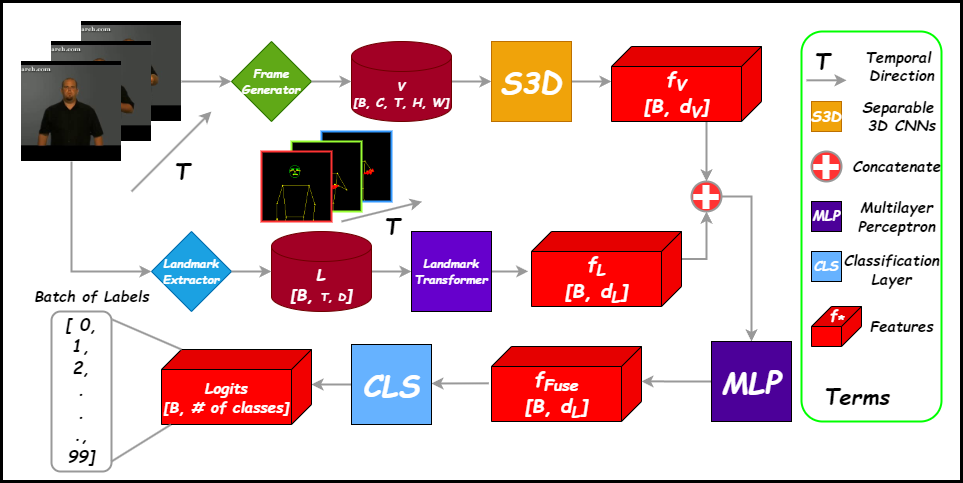
\includegraphics[width=1\linewidth]{Fig/SLNFull.drawio.png}
    \caption{SLN Model Architecture using S3D Backbone and Landmark Transformer (fig \ref{fig:landmark})}
    \label{fig:slnmodel}
\end{figure}

\subsection{Experiments}
To train the SLN model effectively, I selected training configurations for proper performance and ideal computational cost. The number of output classes was set to 100 classes, using the NSLT100 dataset used for SLR. The model was trained with a batch size of 8 and each input sample consisted of a sequence of 64 video frames to capture temporal dynamics. The video frames were resized to 112x112 and 224x224 for more experiments

\vspace{0.5cm}

I ran the training loop for 200 epochs, with early stopping enabled using a patience value of 5 epochs. The learning rate was initialized at $1e-4$ , and Adam optimizer was used with a weight decay of $1e-4$ to prevent overfitting. To manage learning rate adaptation, I chose a Reduce learning rate on plateau scheduler, reducing the learning rate by a factor of $0.5$ if validation loss did not improve over 2 consecutive epochs. Here is Adam formula:

\begin{equation}
\begin{aligned}
m_t &= \beta_1 m_{t-1} + (1 - \beta_1) \nabla L(\theta_t) \\
v_t &= \beta_2 v_{t-1} + (1 - \beta_2) (\nabla L(\theta_t))^2 \\
\hat{m}_t &= \frac{m_t}{1 - \beta_1^t}, \quad \hat{v}_t = \frac{v_t}{1 - \beta_2^t} \\
\theta_{t+1} &= \theta_t - \alpha \frac{\hat{m}_t}{\sqrt{\hat{v}_t} + \epsilon}
\end{aligned}
\end{equation}

\vspace{0.5cm}

where \( \theta_t \) are the model parameters at step \( t \), \( \alpha \) is the learning rate, \( \beta_1 \) and \( \beta_2 \) are exponential decay rates (commonly set to 0.9 and 0.999), and \( \epsilon \) is a small constant (e.g., \( 10^{-8} \)) for numerical stability.

\vspace{0.5cm}

Training phase was on a CUDA-enabled GPU NVIDIA A100 on Google Colab if available, otherwise falling back to CPU. The loss function used was cross-entropy loss, a good option for multi-class classification problems. The loss function used was the \textbf{categorical cross-entropy loss}, defined as:

\begin{equation}
\mathcal{L}_{\text{CE}} = -\sum_{i=1}^{C} y_i \log(\hat{y}_i)
\end{equation}

\vspace{0.5cm}

To ensure efficient GPU usage, auto mixed precision training was an appropriate option . I also applied Gradient clipping to stabilize training and avoid exploding gradients. Additionally, I set a validation phase with 5 steps per training step to lower model computation and Top-5 accuracy was computed during validation to better evaluate the model’s ability to identify the correct label within its top five predictions and required for comparison with SOTA.

\vspace{0.5cm}

Furthermore, I use Tensor Board to track training logs and metrics, enabling visualization of training/validation loss and accuracy curves over time. This configuration ensured a robust and reproducible training pipeline suitable for SLR tasks.

\section{RESULTS AND DISCUSSIONS}

This section is about analyzing the results, comparing with SOTA and discussing the problem.

\subsection{Experimental Results}

For my experiments, the NSTL100 provided training set, consisting of over 2000 videos, was further divided into 3 subsets. The final evaluation of the model’s performance on NSLT100 was conducted as an official test set without external sets.

\begin{figure}[H]
    \centering
    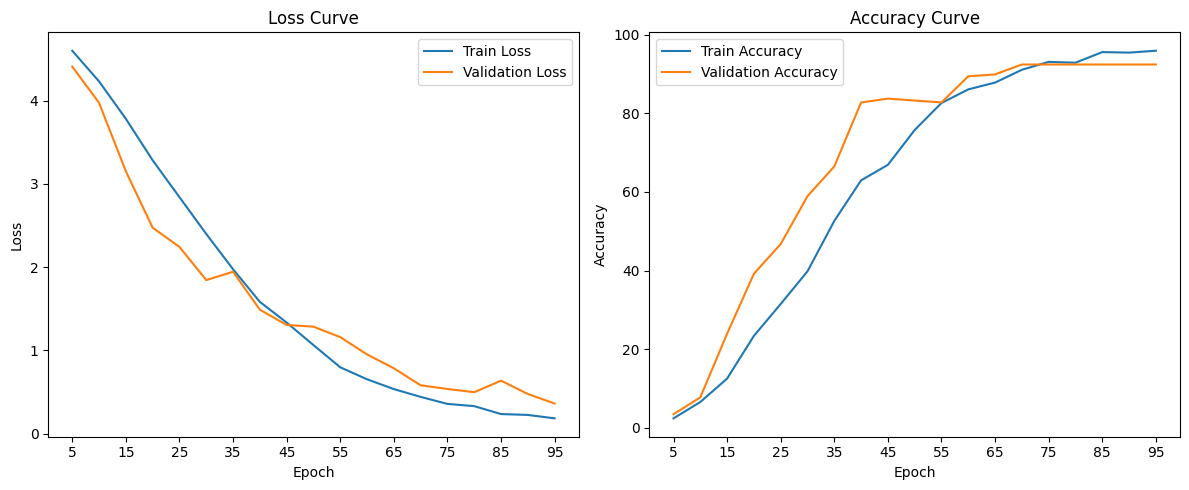
\includegraphics[width=1\linewidth]{Fig/learning_curves.png}
    \caption{Enter Caption}
    \label{fig:learningcurves}
\end{figure}

Through those learning curves, my SLN model is illustrated as a well-performing model and has a great ability to generalize data in the validation phase. SLN achieves Top-1 accuracy at 92.47\% and Top-5 accuracy of 94.92\% on official test set after 95 epochs.

\begin{table}[htbp]
\centering
\label{tab:resolution_comparison}
\begin{tabular}{|c|c|}
\hline
\textbf{Input Resolution} & \textbf{Top-1 Accuracy Per-Instance (\%)}\\
\hline
SLN on 112 × 112 & 72.8  \\
SLN on 224 × 224 & \textbf{92.47} \\
\hline
\end{tabular}
\caption{Comparison of SLN model performance on different input resolutions}
\end{table}

The relustion 224 x 244 significantly outperforms the other ones because the input size of S3D is initialized at 224 x 224.

\vspace{0.5cm}

For further evaluation, I visualized the confusion matrices of Top-10 Performing classes and Bottom-5 Performing classes on the test set.

\begin{figure}[h]
    \centering
    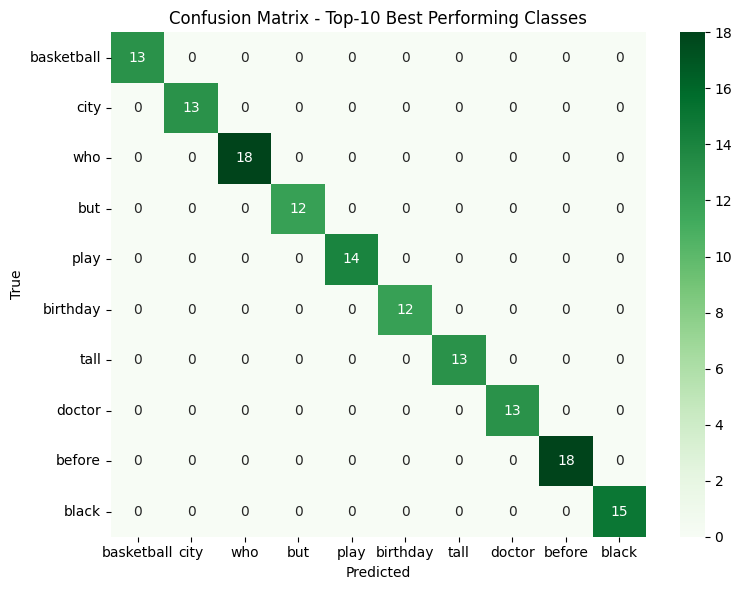
\includegraphics[width=0.85\linewidth]{Fig/top10-acc.png}
    \caption{Top-10 Performing classes}
    \label{fig:top10}
\end{figure}

\begin{figure}[H]
    \centering
    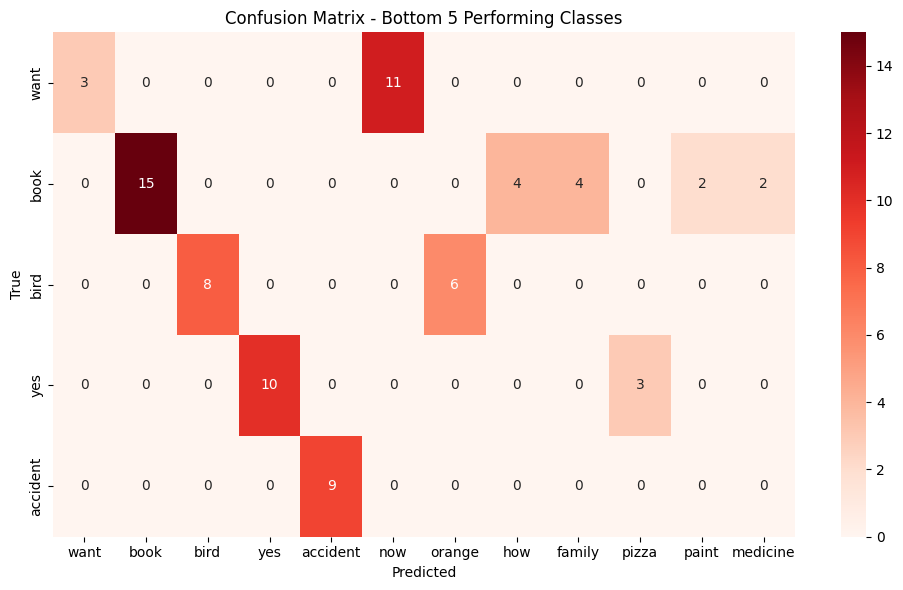
\includegraphics[width=0.9\linewidth]{Fig/bottom5-acc.png}
    \caption{Bottom-5 Performing classes}
    \label{fig:bottom5}
\end{figure}

It is clear to see that all 10 classes Top-10 Performing classes achieve the 100\% accuracy since the high average accuracy per-instance value. In contrast, Bottom-5 Performing classes yield lower results due to mismatch between classes that need to be analyzed.

\begin{table}[htbp]
\centering
\label{tab:bottom5_accuracy}
\begin{tabular}{|c|c|p{8cm}|}
\hline
\textbf{Class} & \textbf{Accuracy (\%)} & \textbf{Misclassifications} \\
\hline
\texttt{want} & 21.43 & now: 11 \\
\hline
\texttt{book} & 50.00 & how: 4, family: 4, paint: 2, medicine: 2, color: 1, fish: 1, all: 1 \\
\hline
\texttt{bird} & 57.14 & orange: 6 \\
\hline
\texttt{yes} & 66.67 & pizza: 3, need: 2 \\
\hline
\texttt{accident} & 69.23 & wrong: 2, fish: 1, language: 1 \\
\hline
\end{tabular}
\caption{Bottom-5 Performing Classes and Misclassification Details}
\end{table}

The main reason for misclassification in the NSLT100 dataset is from the high visual and temporal similarity between certain sign classes. I found that many signs in American Sign Language involve similar hand movement sequence, overlapping spatial locations, and landmarks extracted from those videos are overlapped and share the temporal patterns, which make it challenging for models to discriminate between them especially in cases where the temporal context is short or noisy. Several additional contributing factors include

\begin{itemize}
    \item \textbf{Imbalanced Motion Dynamics:} Some signs have strong dynamic cues (e.g., repetitive hand motion), while others are static or have short durations.
    \item \textbf{Ambiguity in Landmark Representation:} Even with accurate landmark extraction, signs involving overlapping hand-to-face interactions or self-occlusion (such as accident vs. wrong) can produce ambiguous keypoint patterns, reducing classification reliability. 
\end{itemize}

\begin{figure}[H]
    \centering
    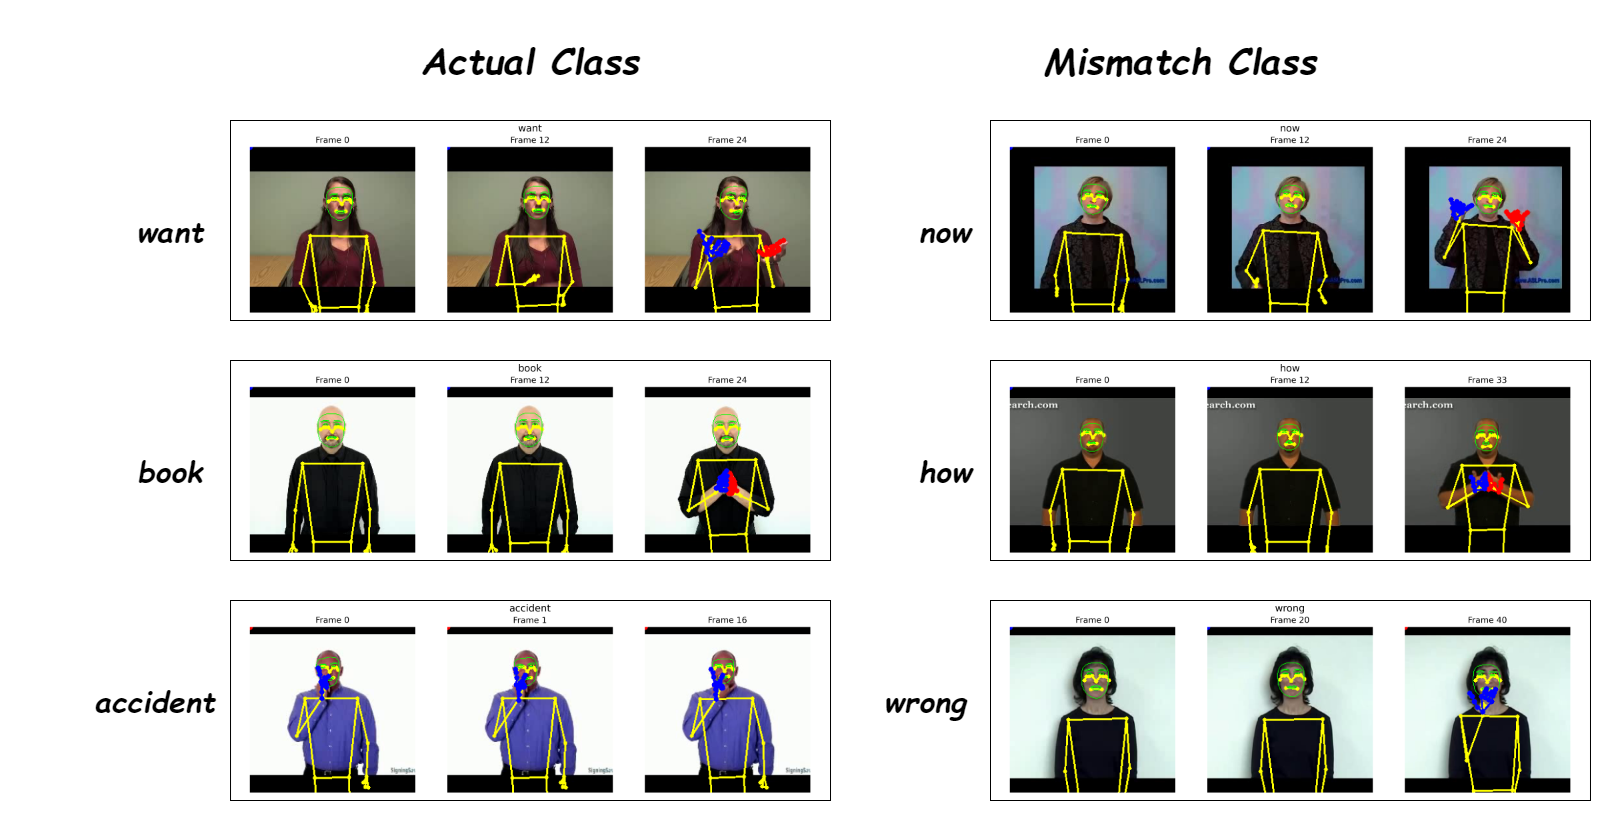
\includegraphics[width=1\linewidth]{Fig/Mismatch.drawio.png}
    \caption{Examples of Misclassification}
    \label{fig:enter-label}
\end{figure}

\subsection{State-of-The-Art}
In this section, I will compare my model performance and accuracy with existing models trained on WLASL100 \cite{paperswithcode_wlasl100} and ranked on paperswithcode.

\begin{table}[H]
\centering
\begin{tabular}{|l|c|c|c|}
\hline
\textbf{Model} & \textbf{Top-1 Acc. (\%)} & \textbf{Params (M)} & \textbf{Year} \\
\hline
UniSign (LLMs Pretrained) \cite{li2025uni-sign} & 92.75 & 679.4 & 2025 \\
NLA-SLR (S3D + VKNet) \cite{zuo2023natural} & 92.64 & --- & 2023 \\
SignBERT \cite{hu2021signbert} & 82.56 & $\sim$110 & 2021 \\
I3D + ST-GCN \cite{maruyama2021wordlevel} & 81.38 & 28.1 & 2021 \\
StepNet \cite{pan2022stepnet} & 78.29 & 194 & 2022 \\
\hline
\textbf{SLN (S3D + Landmark Transformer) [Mine]} & \textbf{92.49} & \textbf{42.3} & 2025 \\
\hline
\end{tabular}
\caption{Comparison of State-of-the-Art Sign Language Recognition Models on WLASL100 Test Set}
\label{tab:sota_comparison}
\end{table}

To prove the uniqueness of my work, I would like to compare my results to other interns that focus on the same topic.

\renewcommand{\arraystretch}{1.4}
\begin{table}[htbp]
\centering
\begin{tabular}{|c|c|c|c|c|}
\hline
\textbf{Name} & \textbf{Dataset} & \textbf{Preprocess} & \textbf{Input Size} & \textbf{Model}\\
\hline
\makecell{Le Duy Anh \\ 22BI13017-DS} & \makecell{WLASL2000 \\ MSASL2000} & \makecell{Extract bones \\ frames using \\ RTMPose FrameWork} & \makecell{64x3x224x224} & \makecell{Pretrain Tranformers and \\ Mask Modeling \\ to get weights, \\ Integrate on Unisign}\\
\hline
\makecell{Nguyen Hoang Minh \\ 22BI13291-ICT} & NSLT100 & \makecell{Extract bones \\ frames using \\ OpenPose FrameWork} & \makecell{64x3x224x224} & \makecell{Layers of GCN \\ for extract number \\ of keypoint with \\ number of hidden layers, \\ layers GCN to \\ determine words, \\ RNN layers to \\ connect frames}\\
\hline
\textbf{\makecell{Le Duc Dung\\(Me)}} & NSLT100 & \makecell{Frame Generation \\ to generate 64 \\ frames per videos, \\ resize each frame \\ to 224x224, Landmarks \\ Extraction using \\ Mediapipe Holistic} & \makecell{64x3x224x224 \\ (videos) \\ 64x543x3 \\ (landmarks)} & \makecell{S3D for video \\ features extraction \\ and Landmark \\ Transformer for \\ sequence of landmarks}\\
\hline
\end{tabular}
\caption{Comparison between Interns - Methodology}
\label{tab:intern_comparison_method}
\end{table}

\renewcommand{\arraystretch}{1.4}
\begin{table}[H]
\centering
\begin{tabular}{|c|c|c|c|c|}
\hline
\textbf{Name} & \textbf{Dataset} & \textbf{\makecell{Execution time \\ Full pipeline}} & \textbf{\makecell{\#Param(M)}} & \textbf{\makecell{Top-1 \\ Acc. Per-i}}\\
\hline
\makecell{Le Duy Anh \\ 22BI13017-DS} & \makecell{WLASL2000 \\ MSASL2000} & \makecell{6 hours} & 317.8 & 58\% \\
\hline
\makecell{Nguyen Hoang Minh \\ 22BI13291-ICT} & NSLT100 & \makecell{6 hours} & 6 & 64.62\% \\
\hline
\textbf{\makecell{Le Duc Dung \\ (Me)}} & \textbf{NSLT100} & \makecell{\textbf{2.5 hours}} & \textbf{42.3} & \textbf{92.49\%} \\
\hline
\end{tabular}
\caption{Comparison between Interns - Results}
\label{tab:intern_comparison}
\end{table}

\subsection{Discussion}

This section reflects on the methods I employed throughout my research, taking a closer look at what worked well and where there were limitations. 

\vspace{0.5cm}

The results of this study highlight the effectiveness of the proposed SLN model, which combines visual features from S3D with structural information from the Landmark Transformer. With a Top-1 accuracy of 92.49\% on the NSLT100 dataset, my model performs competitively compared to several SOTA approaches and can outperform many models. This indicates that integrating temporal-spatial representations with full-body landmarks can significantly enhance SLR performance.

\vspace{0.5cm}

One important observation is that the model trained on input resolution of 224×224 achieved much higher accuracy than when trained on 112×112. This suggests that preserving finer details in both the video frames and landmark features improves the model’s ability to recognize between similar signs.

\vspace{0.5cm}

Despite strong overall performance, I made a closer analysis of the confusion matrices and it revealed several misclassifications, particularly in classes with overlapping signs. For example, the sign “want” was frequently confused with “now,” and “book” was often misclassified as “how” or “family.” I believe some of the mistakes in prediction happened because the model wasn’t always able to catch small differences in hand movements or facial expressions. These details are sometimes too fine for the current landmark features to represent well. This made me realize that having a more diverse set of training examples and improving how the landmarks are captured could really help. With better data and more precise landmark extraction, the model might understand those hard-to-distinguish signs more clearly.

\vspace{0.5cm}

Overall, the experimental results validate that combining raw video data features extracted by S3D backbone \cite{xie2017rethinking} with structured landmark can lead to a robust and well-performed model.

\section{CONCLUSION}

In this section, I will make a conclusion about my thesis, limitations and future works to improve and complete them.

\subsection{Conclusion}
In this research, I succeed to build my own SLN model which is a fused model between S3D backbone and Landmark Transformer. By training this model on NSLT100 dataset, I achieve Top-1 accuracy of 92.49\% on official test set and reach top 3 in the SOTA comparison table (table \ref{tab:sota_comparison}) in many aspects such as accuracy and model weight. With SLN model, I fulfilled my stated objectives in this research and gained many experiences in processing raw video data, extracting landmarks with tools and transfer learning technique.

\subsection{Limitations}
Despite the high accuracy and strong performance, my SLN model shows several limitations. Addressing overlapping signs and videos with short duration are two main reasons that make SLN struggle to recognize sign and yield poor results. In addition, bigger datasets will be a difficult challenges for this model to learn and generalize due to current setups and architecture. These areas might need more investigation and improvement on pre-processing techniques and model constructing to address existing limitations above.

\subsection{Future Works}
While my SLN model has demonstrated strong performance in recognizing sign language, I believe there is more room for meaningful improvements. One idea I’m particularly interested in exploring is the use of more detailed landmark data, especially in areas like the face and fingers. These regions often result overlaps that can make a big difference when distinguishing between similar signs. I also noticed that the model might struggle a bit with signs that vary across different individuals, so expanding the dataset to include more diverse signers could be an important step forward. This would not only improve generalization but also make the model more inclusive and robust in real-world scenarios. Moreover, training and evaluating model with other sign language and bigger dataset such as WLASL2000 will be my next future work to improve model performance and enhance the model architect for better recognition between signs.Finally, from a practical point of view, I see a lot of value in optimizing the model so it can run efficiently on edge devices like smartphones or tablets. This would make it more accessible and useful in everyday situations, especially for real-time applications such as sign language translation tools. I believe that making the model more inclusive and user-focused is just as important as improving its accuracy.

\newpage
%------------------------------END OF DOCUMENTS-----------------------------%
% References
\addcontentsline{toc}{section}{REFERENCES}
%\begin{multicols}{2}
\printbibliography
%\end{multicols}

\end{document}
